\documentclass[a4paper,12pt,titlepage=false]{scrreprt}

\usepackage[ngerman]{babel}
\usepackage[utf8]{inputenc}
\usepackage[a4paper, left=2cm, right=2cm, top=1.5cm, bottom=2cm]{geometry}
\usepackage{graphicx}
\usepackage{wrapfig}
\usepackage{setspace}
\usepackage{tikz}
\usepackage{stmaryrd}
\usepackage{listings}
\usepackage{amsmath}
\usepackage{chngcntr}
\usepackage{textcomp}
\usepackage[hidelinks]{hyperref}

\usetikzlibrary{positioning}
\usetikzlibrary{arrows}
\tikzstyle{block} = [rectangle, draw, text width=7em, text centered, rounded corners, minimum height=4em]
\tikzstyle{line} = [draw, -latex']

\definecolor{light-gray}{gray}{0.6}

\titlehead{Seminar: Anwendungen Linguistische Informatik \hfill Vortrag am 06.07.2015}
\title{\vspace{3cm}Common Crawl}
\subtitle{Analyse des Crawling-Prozesses und der Textextraktion}
\author{Klemens Schölhorn \and Erik Körner \and Kai Hainke}

% show toc on titlepage
\setuptoc{toc}{leveldown}

% no page number on titlepage
\renewcommand*{\titlepagestyle}{empty}

% continuous numbering of footnotes
\counterwithout{footnote}{chapter}

\begin{document}

\maketitle
\vspace{2cm}
\tableofcontents

\onehalfspacing

\chapter{Common Crawl}

\textbf{``Our goal is to democratize the data so everyone, not just big companies, can do high quality research and analysis.''}
\hfill-- \textit{Common Crawl Foundation}

\section{Organisation}

Common Crawl ist eine 2007 durch Gil Elbaz gegründete gemeinnützige Organisation mit dem Ziel, Wissenschaftlern, Firmen und Privatpersonen kostenlos eine Kopie des Internets zu Forschungs- und Analysezwecken zur Verfügung zu stellen\footnote{\url{https://commoncrawl.org/faqs/}}.

Dazu wird monatlich ein Crawl erstellt, der anschließend in einem AWS Public Data Set\footnote{\url{https://aws.amazon.com/datasets/41740}} von Amazon kostenfrei gespeichert wird. Dies ermöglicht die direkte Analyse in AWS, aber auch den freien Download über HTTP.

Die Organisation hat zur Zeit 25 Mitglieder, wobei die Mehrzahl Fachwissen und Zeit unentgeltlich zur Verfügung stellen.

\section{Technik}

Common Crawl verwendet für das Crawlen den CCBot, einen modifizierten Apache Nutch 1.7, welcher wiederum auf Lucene, Solr und Hadoop basiert. Das Crawlen findet verteilt in AWS statt. Der CCBot beachtet die \texttt{robots.txt} und versucht durch einen ausgeklügelten Algorithmus so wenig Last wie möglich auf den einzelnen Webservern zu verursachen.

Zur Speicherung der Crawls wird das Web Archive-Format (WARC) verwendet, das in ISO 28500\footnote{\url{http://bibnum.bnf.fr/WARC/WARC_ISO_28500_version1_latestdraft.pdf}} spezifiziert und an HTTP angelehnt ist. Eine WARC-Datei besteht aus mehreren einzelnen WARC-Records, wobei ein WARC-Record einen beliebigen Payload haben kann (z.\,B. HTTP oder JSON).

Während des Crawls werden drei verschiedene Ergebnisse erzeugt: Zuerst der Crawl an sich mit den kompletten HTTP-Konversationen, wobei Anfrage und Antwort als getrennte WARC-Records abgespeichert werden. Zusätzlich wird für jeden WARC-Record ein JSON-Metadaten-Record\footnote{\url{https://gist.github.com/Smerity/e750f0ef0ab9aa366558\#file-bbc-pretty-wat}} (WAT) erzeugt, der u.\,a. die kompletten HTTP-Header sowie eine Liste aller auf der Seite vorkommenden Links (inklusive der eingebundenen CSS/JavaScript-Dateien) enthält. Schließlich wird für jede HTTP-Antwort auch ein Reintext-Record (WET) erzeugt, der den automatisch aus dem HTML-Quelltext extrahierten Text enthält.


\chapter{Analyse}

Die Analyse erfolgte anhand des Crawls vom April 2015, des zum Zeitpunkt des
Vortrages aktuellsten Crawls. Der komplette Crawl besitzt eine Größe von 168 TB und beinhaltet 2,1 Milliarden Webseiten\footnote{\url{http://blog.commoncrawl.org/2015/05/april-2015-crawl-archive-available/}}.
Da eine Bearbeitung dieser Datenmenge auf eigenen Servern aufgrund von
Bandbreitenbeschränkungen und eine Bearbeitung in AWS mit Hilfe von EC2-Instanzen
aufgrund von finanziellen Einschränkungen nicht möglich war, haben wir unsere
Analyse auf die WAT-Dateien beschränkt, die aus knapp 39000 Dateien zu
durchschnittlich je 315 MiB bestehen und damit zusammen nur rund 12 TB groß sind.
Davon konnten wir ca. 53 \% analysieren.

\section{Übersicht}

\begin{wrapfigure}{r}{.54\textwidth}
\label{wrap-fig:1}
\begin{tikzpicture}[auto]
    \node[block] (CC) at (0,0) {Common Crawl};
    \node[block, right=3.5cm of CC] (META) {meta-extractor};
    \node[block, below=1.5cm of META] (MONET) {MonetDB};
    \node[block, left=3.5cm of MONET] (R) {R};
    \path[line] (CC) -- node {Download (curl)} (META);
    \path[line] (META) -- node {csv} (MONET);
    \path[line] (MONET) -- node {MonetDB.R} (R);
\end{tikzpicture}
\end{wrapfigure}

Die nebenstehende Abbildung zeigt den strukturellen Ablauf der Analyse.

Der Download und die Extraktion der benötigten Daten mit Hilfe des
\texttt{meta-extractor}s erfolgte parallel auf dem zur Verfügung gestellten
Praktikumsrechner und auf einem privaten Server eines Autors. Dabei wurden keine
Dateien lokal zwischengespeichert, sondern die WAT-Dateien mittels Unix-Pipes
direkt von \texttt{curl} in den \texttt{meta-extractor} und anschließend die
resultierenden csv-Dateien mittels \texttt{ssh} direkt auf den genannten
privaten Server zur weiteren Analyse geladen.

Dazu wurden die Daten in die spaltenorientierte Datenbank
\texttt{MonetDB}\footnote{\url{https://www.monetdb.org/}} importiert, um
anschließend mittels der \texttt{R}-Anbindung darauf in \texttt{R} Analysen
durchführen zu können.

\section{\texttt{meta-extractor}}

Der \texttt{meta-extractor} ist ein in \texttt{C++} geschriebenes Programm,
das sequentiell Metadaten-WARC-Records aus WAT-Dateien auslesen und daraus
die im Abschnitt \ref{csv-data} beschriebenen Metadaten als csv-Datei extrahieren
kann.

Dazu wurden neben einem csv-Writer ein standardkonformer WARC-Parser und eine
Trie-Implementierung für den effizienten Lookup des \texttt{Public Suffix} einer
Domain aus der \texttt{Public Suffix}-Liste\footnote{\url{https://publicsuffix.org/}} implementiert. Außerdem wurde auf RapidJSON\footnote{\url{https://github.com/miloyip/rapidjson}}
zum schnellen Parsen der WAT-Metadaten, auf die URI-Klasse des
POCO-Projektes\footnote{\url{http://pocoproject.org/}} und auf
TCLAP\footnote{\url{http://tclap.sourceforge.net/}} für das CLI zurückgegriffen. Das Test-Framework Catch\footnote{\url{https://github.com/philsquared/Catch}} wurde für Unit-Tests der selbst geschriebenen Komponenten und für Integrationstests verwendet.

Das beiliegende \texttt{Makefile} ist für den \texttt{GCC C++}-Compiler konzipiert, der Code lässt sich jedoch mit jedem standardkonformen \texttt{C++11}-Compiler übersetzen.

\section{Hilfsmittel}

Neben dem \texttt{meta-extractor} wurden noch einige Skripte u.\,a. zur
Steuerung des Downloads und der Extraktion, dem Import in \texttt{MonetDB} und
der Analyse in \texttt{R} geschrieben. Das erste Skript ist etwas umfangreicher
und daher neben dem Hauptprogramm auch Teil des
Projektrepositories\footnote{\url{https://github.com/klemens/ALI-CC/}}.

\section{Gesammelte Metadaten}
\label{csv-data}

Die in folgender Tabelle beschriebenen Metadaten wurden vom \texttt{meta-extractor}
extrahiert und für die weiteren Analysen verwendet:

\begin{center}
\begin{tabular}{lcl}
    \textbf{Name}  & \textbf{Datentyp} & \textbf{Beispiel} \\ \hline\hline
    UUID           & uint128           & \textcolor{light-gray}{14a939f4-2355-11e5-b5f7-727283247c7f} \\ \hline
    Zeitstempel    & string            & \textcolor{light-gray}{2015-07-06T11:03:18T} \\ \hline
    Verwendung TLS & bool              & https ja/nein \\ \hline
    Hostname       & string            & \textcolor{light-gray}{amazon.co.uk} \\ \hline
    TLD            & string            & \textcolor{light-gray}{uk} \\ \hline
    Public Suffix  & string            & \textcolor{light-gray}{co.uk} \\ \hline
    Pfadtiefe      & uint8             & \textit{test/cool/cool.html} $\rightarrow$ \textcolor{light-gray}{3} \\ \hline
    Pfadlänge      & uint16            & \textit{test/cool/cool.html} $\rightarrow$ \textcolor{light-gray}{19} \\ \hline
    Server         & string            & \textcolor{light-gray}{apache}, \textcolor{light-gray}{nginx}, \dots \\ \hline
    Kompression    & bool              & \textcolor{light-gray}{gzip}, \textcolor{light-gray}{deflate} in \textit{Content-Encoding} \\ \hline
    Cookies        & bool              & \textit{Set-Cookie} vorhanden \\ \hline
    MIME-Typ       & string            & \textcolor{light-gray}{text/html}, \textcolor{light-gray}{application/xml}, \dots\\ \hline
    Charset        & string            & \textcolor{light-gray}{utf}, \textcolor{light-gray}{iso-8859}, \dots \\ \hline
    Verwendung CDN & bool              & CDN ja/nein \\ \hline
    Interne Links  & uint16            & Anzahl relativer Links + gleicher Host \\ \hline
    Externe Links  & uint16            & Anzahl ausgehender Links
\end{tabular}
\end{center}


\chapter{Ergebnisse}

\section{Top-Level-Domain}

\begin{center}
    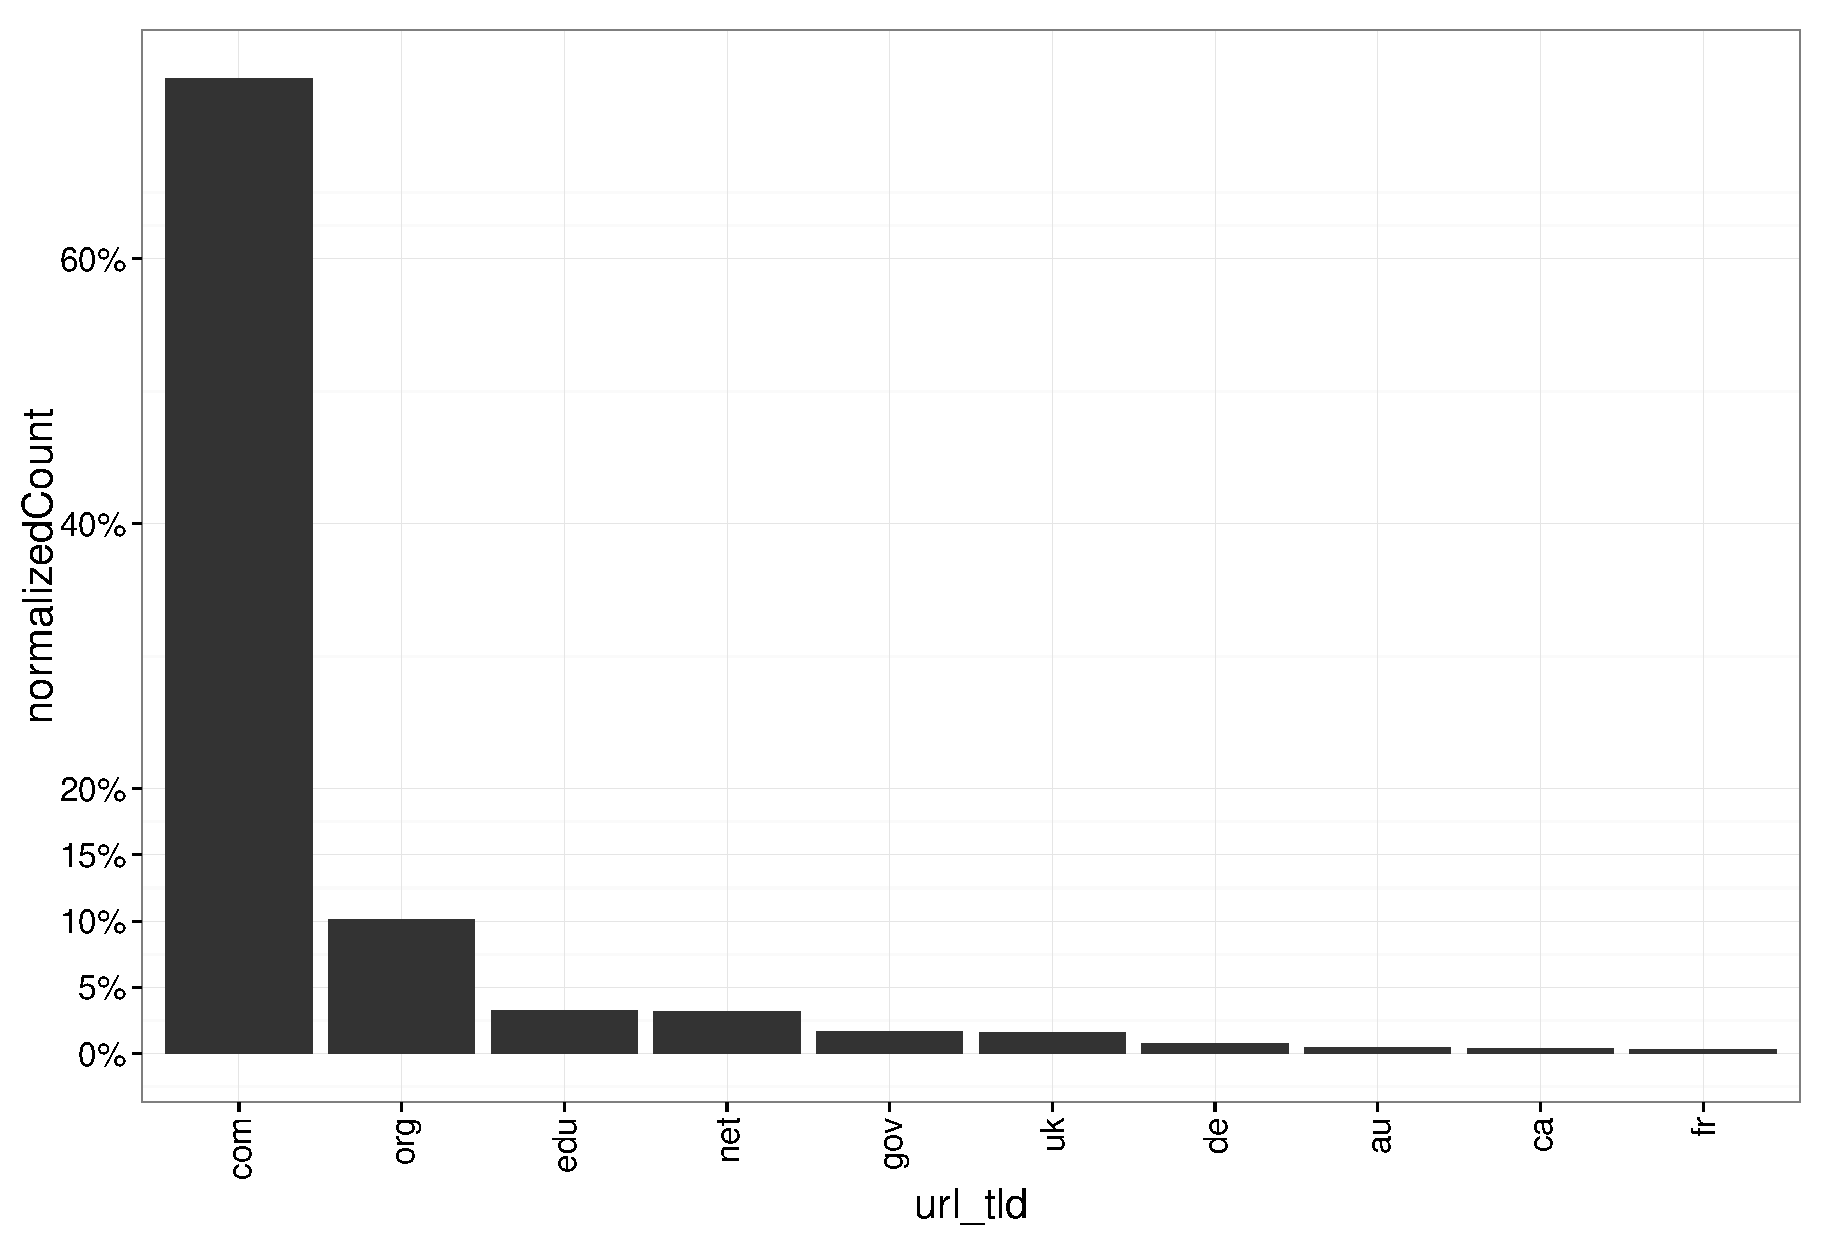
\includegraphics[width=0.9\textwidth]{plots/plot_tld_top10}
\end{center}

\noindent
Die TLD .com, die vor allem von kommerziellen Unternehmen genutzt wird, ist mit über 70\% mit Abstand am meisten vertreten. Danach folgt die eher von nicht-kommerziellen Organisationen benutzte .org.

\begin{wrapfigure}{r}{.63\textwidth}
    \label{wrap-fig:2}
    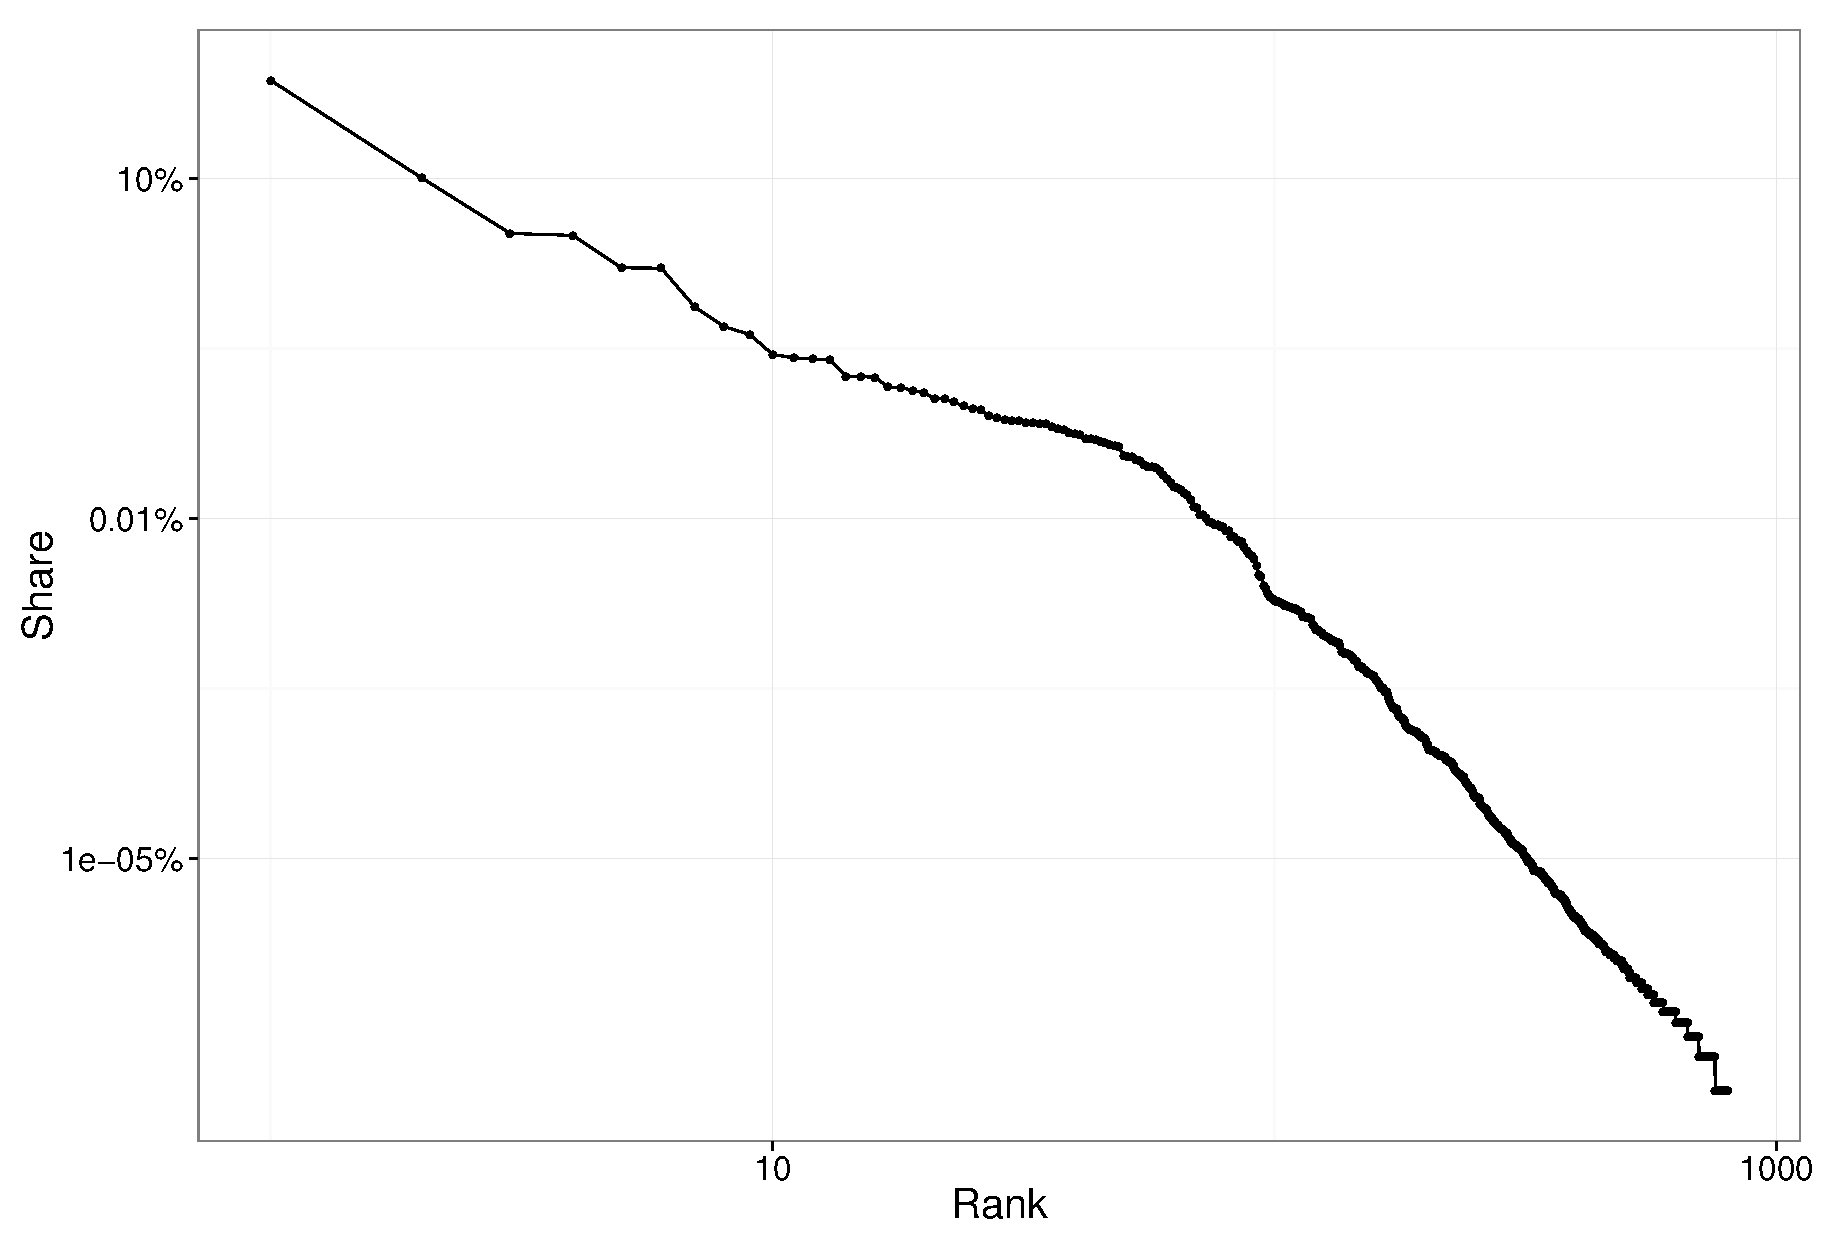
\includegraphics[width=.63\textwidth]{plots/plot_tld_zipf}
\end{wrapfigure}

Mit .edu und .gov befinden sich zwei TLDs unter den Top-5, die primär von US-amerikanischen Bildungs- und Regierungsorganisationen verwendet werden. Anschließend folgen länderspezifische TLDs, wobei englischsprachige und europäische Länder den überwiegenden Anteil stellen.

Grundsätzlich scheinen die TLDs näherungsweise zipfverteilt zu sein.

% prevent wrapfigure from floating into next pages
\clearpage

\begin{wrapfigure}{r}{.45\textwidth}
    \label{wrap-fig:3}
    \def\svgwidth{.45\textwidth}
    \input{images/selection_bias_clean.pdf_tex}
\end{wrapfigure}

Die von Common Crawl erfassten Seiten stellen eine nicht randomisierte Stichprobe aus der Gesamtheit aller Websites dar. Daher unterliegen die Ergebnisse einer statistischen Verzerrung im Vergleich zur wahren Verteilung der Grundgesamtheit aller Websites, dem Selection Bias. Um abzuschätzen, in wie weit die Auswahl von Websites durch den Common Crawl-Prozess im Vergleich zu einer randomisierten Auswahl verzerrt ist, vergleichen wir die Verteilung der TLDs mit Daten von Google. Auch diese Daten unterliegen natürlich dem Selection Bias, haben aber eine größere Stichprobengröße.

Da Google selbst keine offiziellen Statistiken über die erfassten TLD bereitstellt, wurden die Daten über eine speziell formulierte Suchanfrage der Form \texttt{site:.com} erhoben. Dies liefert alle Seiten, die in Ihrer Domain den String .com enthalten, was näherungsweise alle Seiten der TLD .com sind. Auf diese Weise wurden die Trefferzahlen der 61 häufigsten Domains ermittelt und in Relation zueinander gesetzt. Aufgrund der nicht vollständigen Abdeckung aller TLDs sind die relativen Anteile geringfügig zu hoch.

\begin{center}
    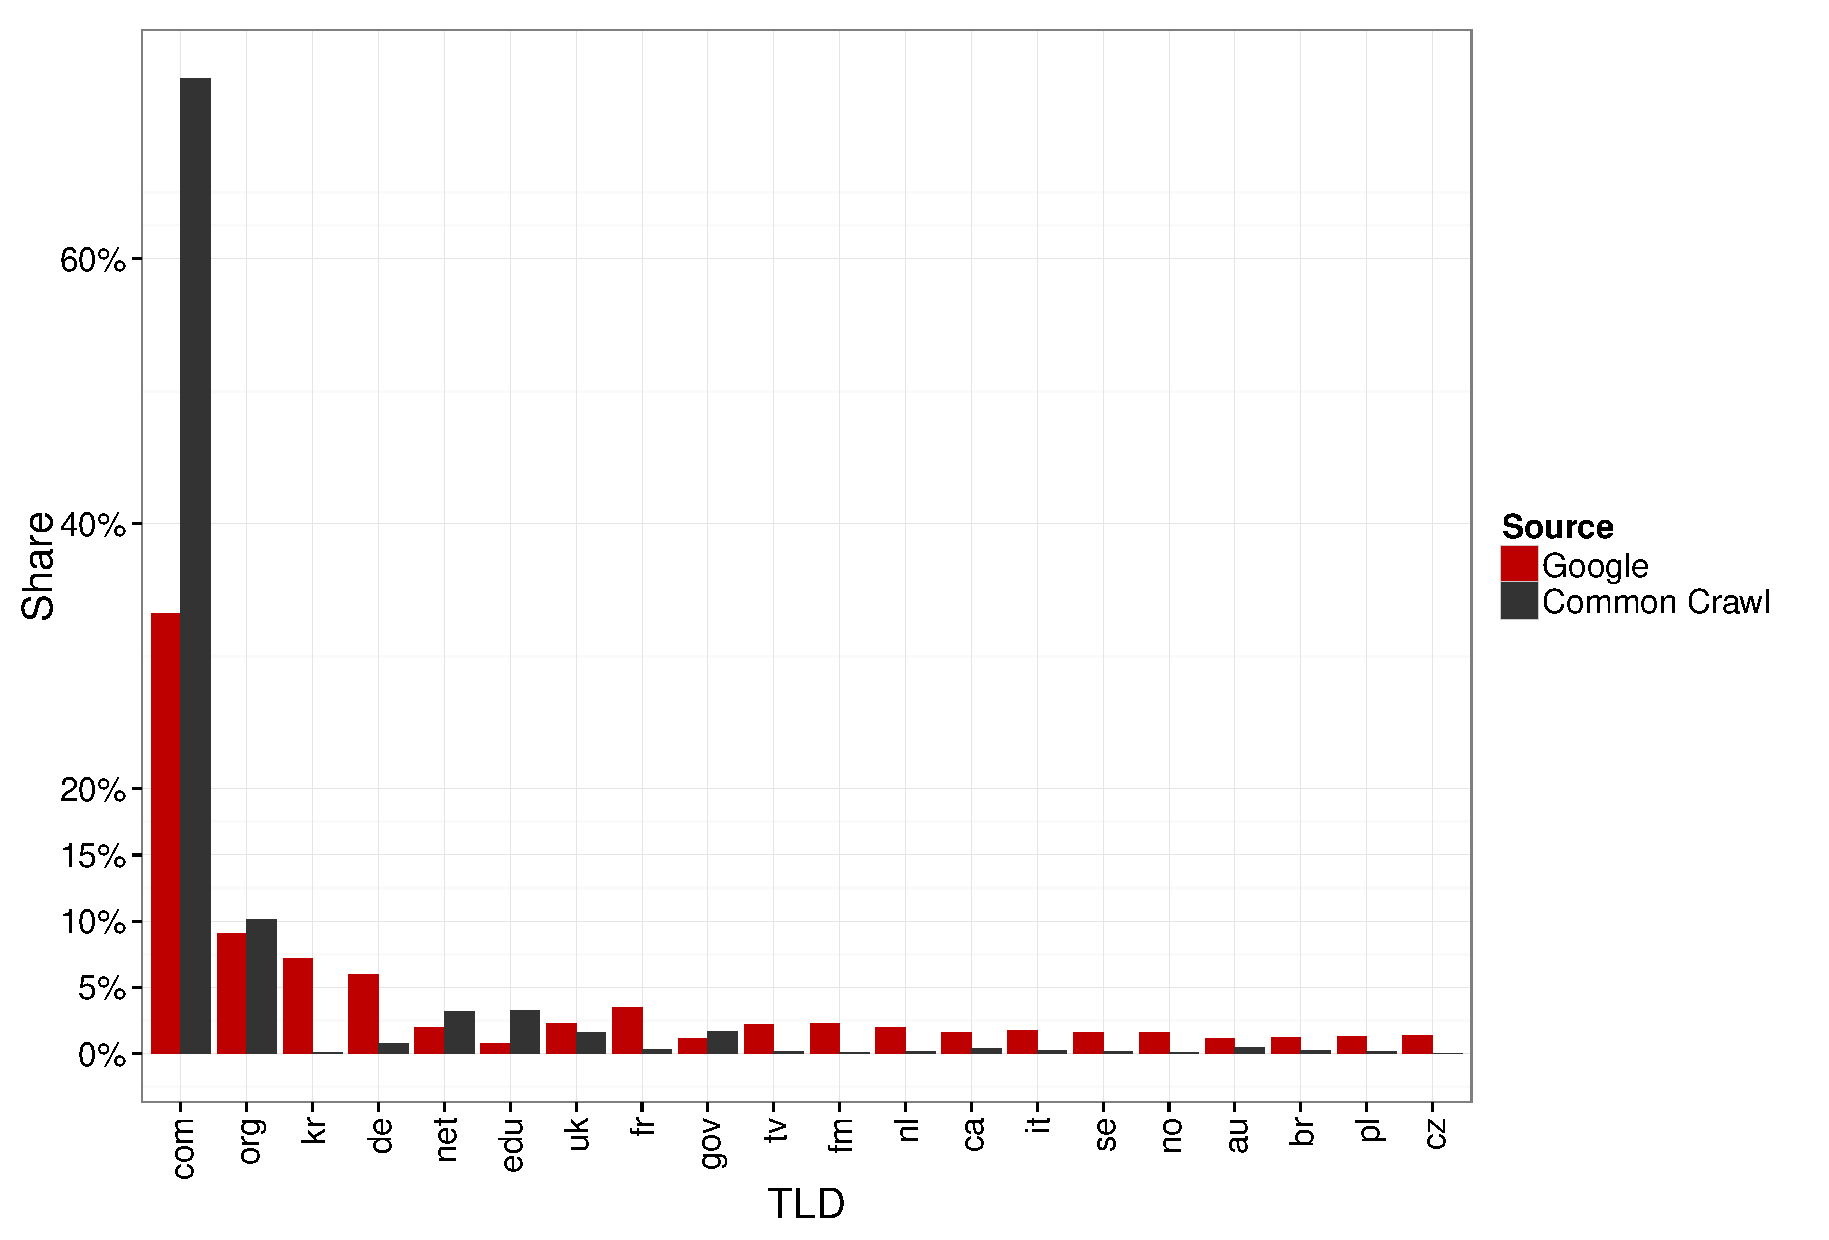
\includegraphics[width=.9\textwidth]{plots/plot_tld_comparison}
\end{center}

Es zeigt sich, dass mit Ausnahme englischsprachiger Länder (besonders asiatische) länder-spezifische TLDs stark unterrepräsentiert sind (z.\,B. Südkorea .kr), während amerikanische TLDs (.edu, .gov) und die kommerzielle TLD .com stark überrepräsentiert sind. Typische TLDs von Websites für Medienstreaming (z.\,B. .tv und .fm) sind ebenfalls unterrepräsentiert.

\section{Public Suffix}

\begin{center}
    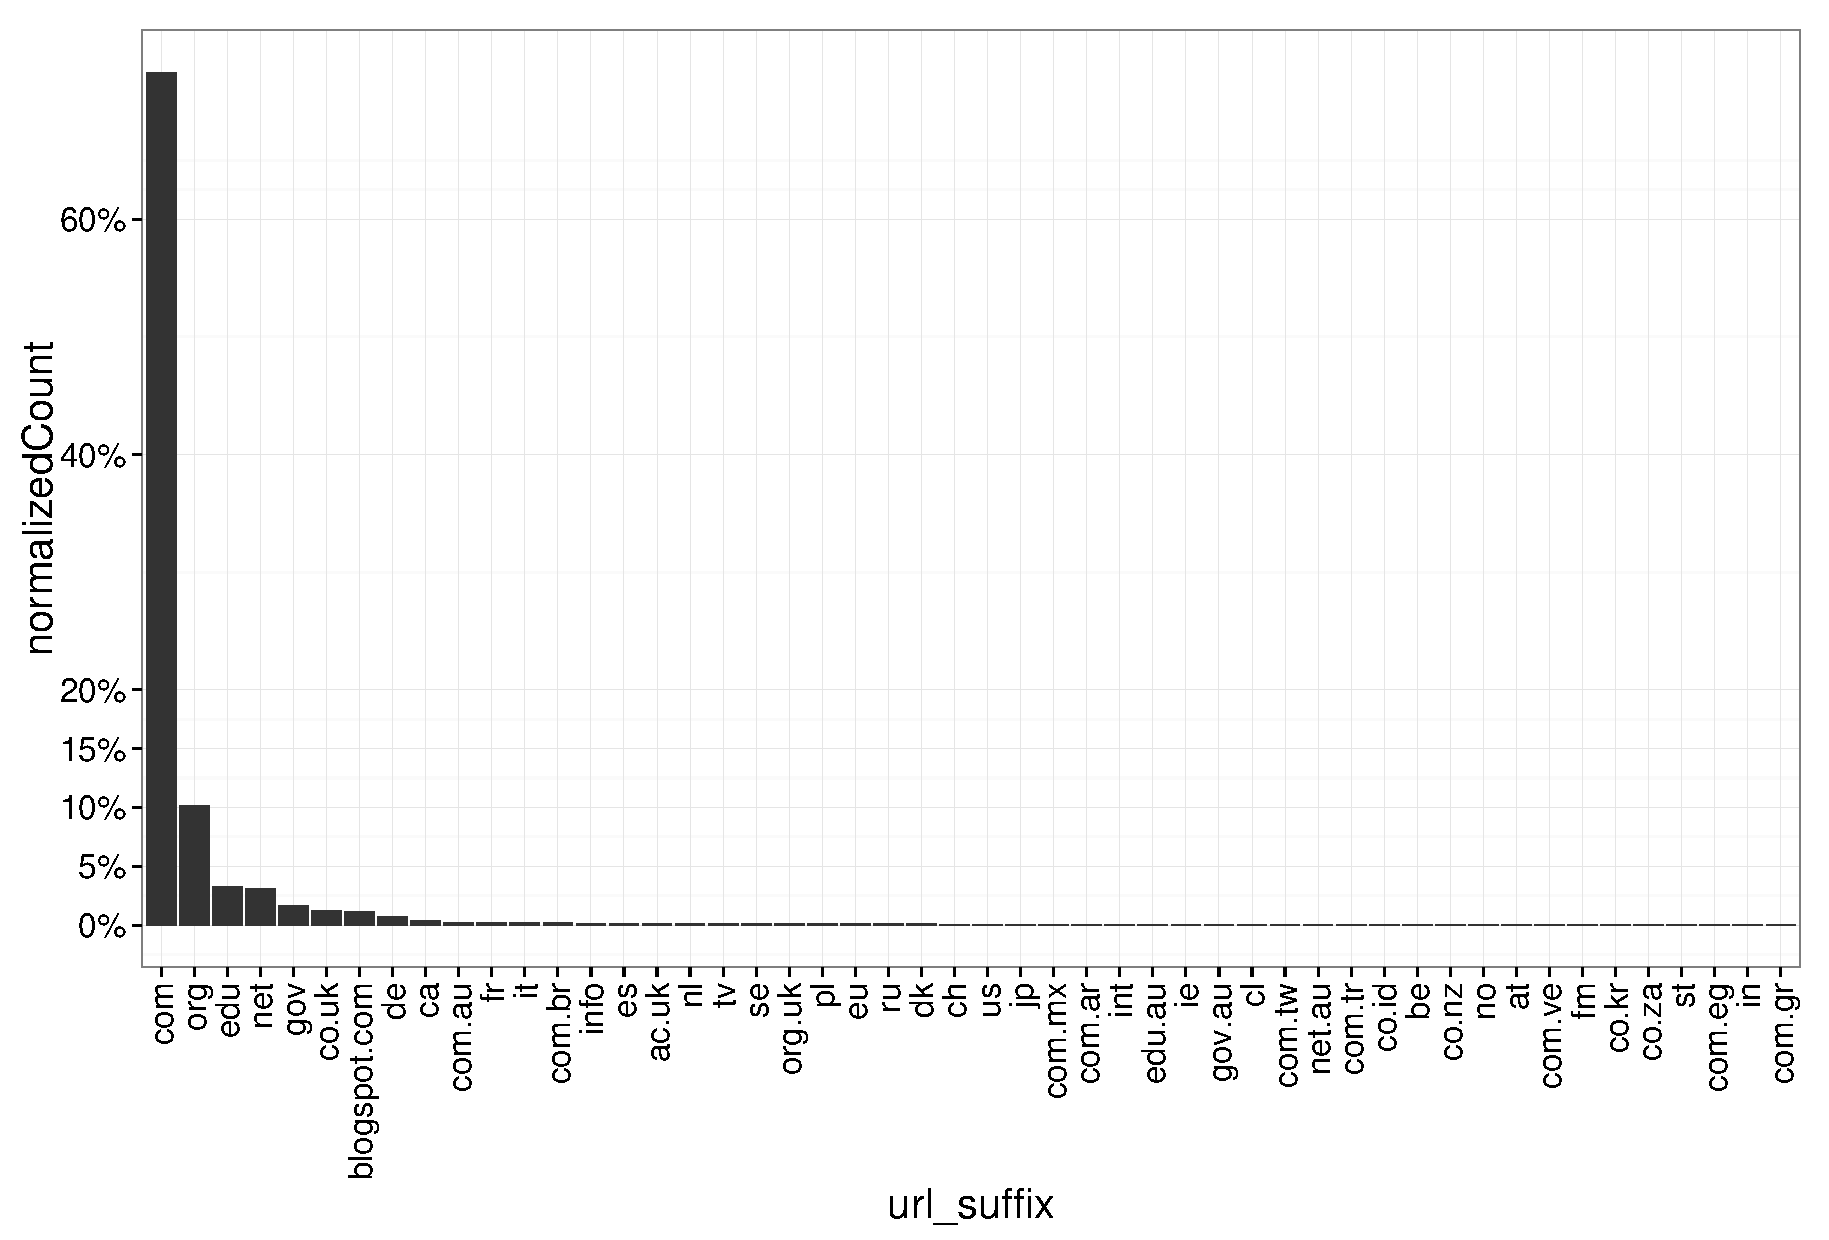
\includegraphics[width=.9\textwidth]{plots/plot_pub_suffixes_top50}
\end{center}

\noindent
Wie zu erwarten zeigt sich bei den Public Suffixes ein ähnliches Bild wie bei den TLDs. Ein extremer Ausreißer ist der Blog-Dienst blogger.com mit seinen auf blogspot.com gehosteten Blogs.

Außerdem erscheinen nun z.\,B. .co.uk, .org.uk, etc. weit vor .uk (nicht im Graph), da die Registrierung von Domains direkt unter .uk erst seit kurzem erlaubt und damit noch nicht weit verbreitet ist.

\section{Mime-Type}

\begin{wrapfigure}{r}{.6\textwidth}
    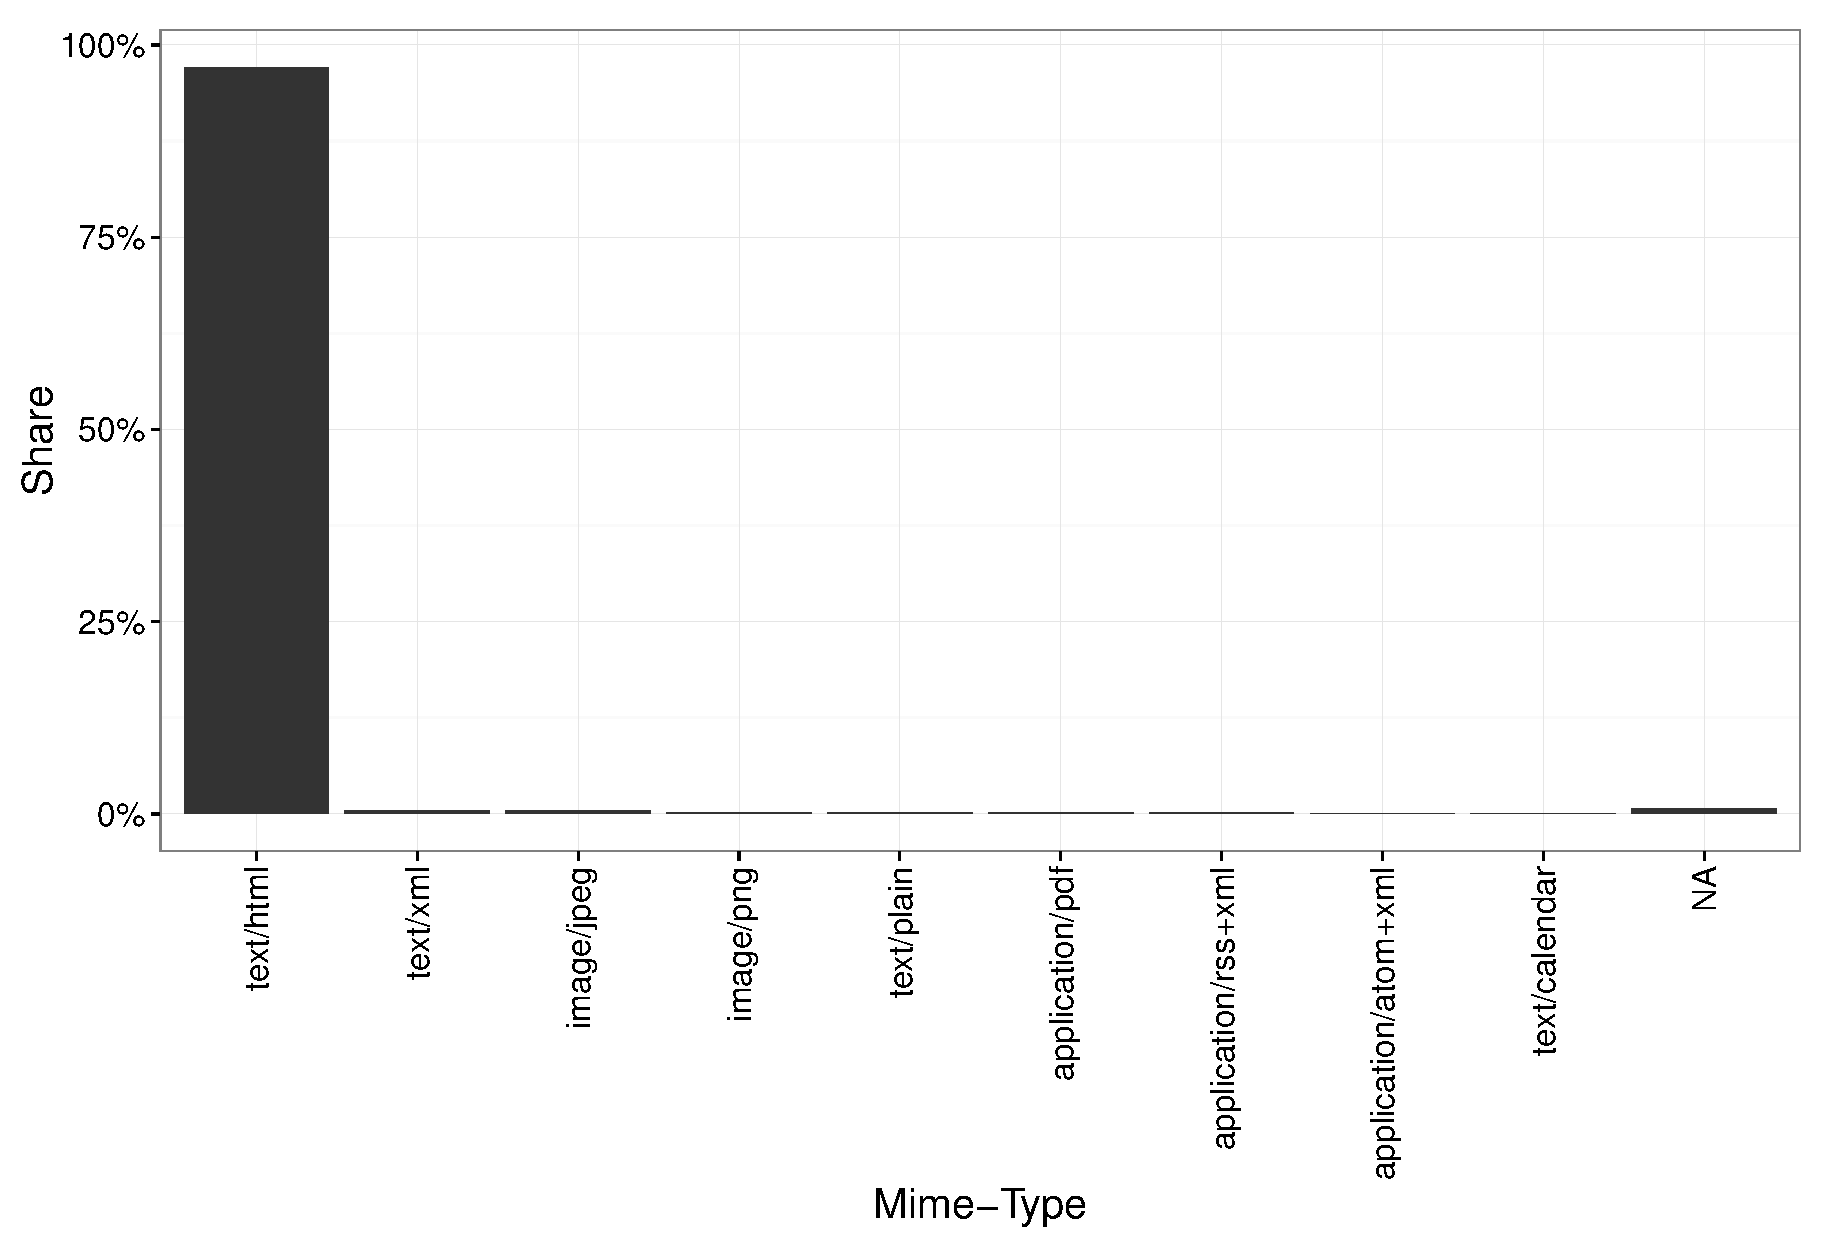
\includegraphics[width=.6\textwidth]{plots/plot_mime}
\end{wrapfigure}

Es werden fast ausschließlich HTML-Textdaten gecrawlt, was den Erwartungen entspricht. Andere typische gecrawlte Typen sind Bilder, PDFs, Feeds und Kalender.

Da die eigentlichen Daten nicht analysiert wurden und die HTTP-Header möglicherweise nicht immer korrekt sind (z.\,B. falsch konfigurierter Webserver), sollten diese Daten kritisch gesehen werden.

% prevent wrapfigure from floating into next pages
\clearpage

\section{Zeichenkodierung}

\begin{center}
    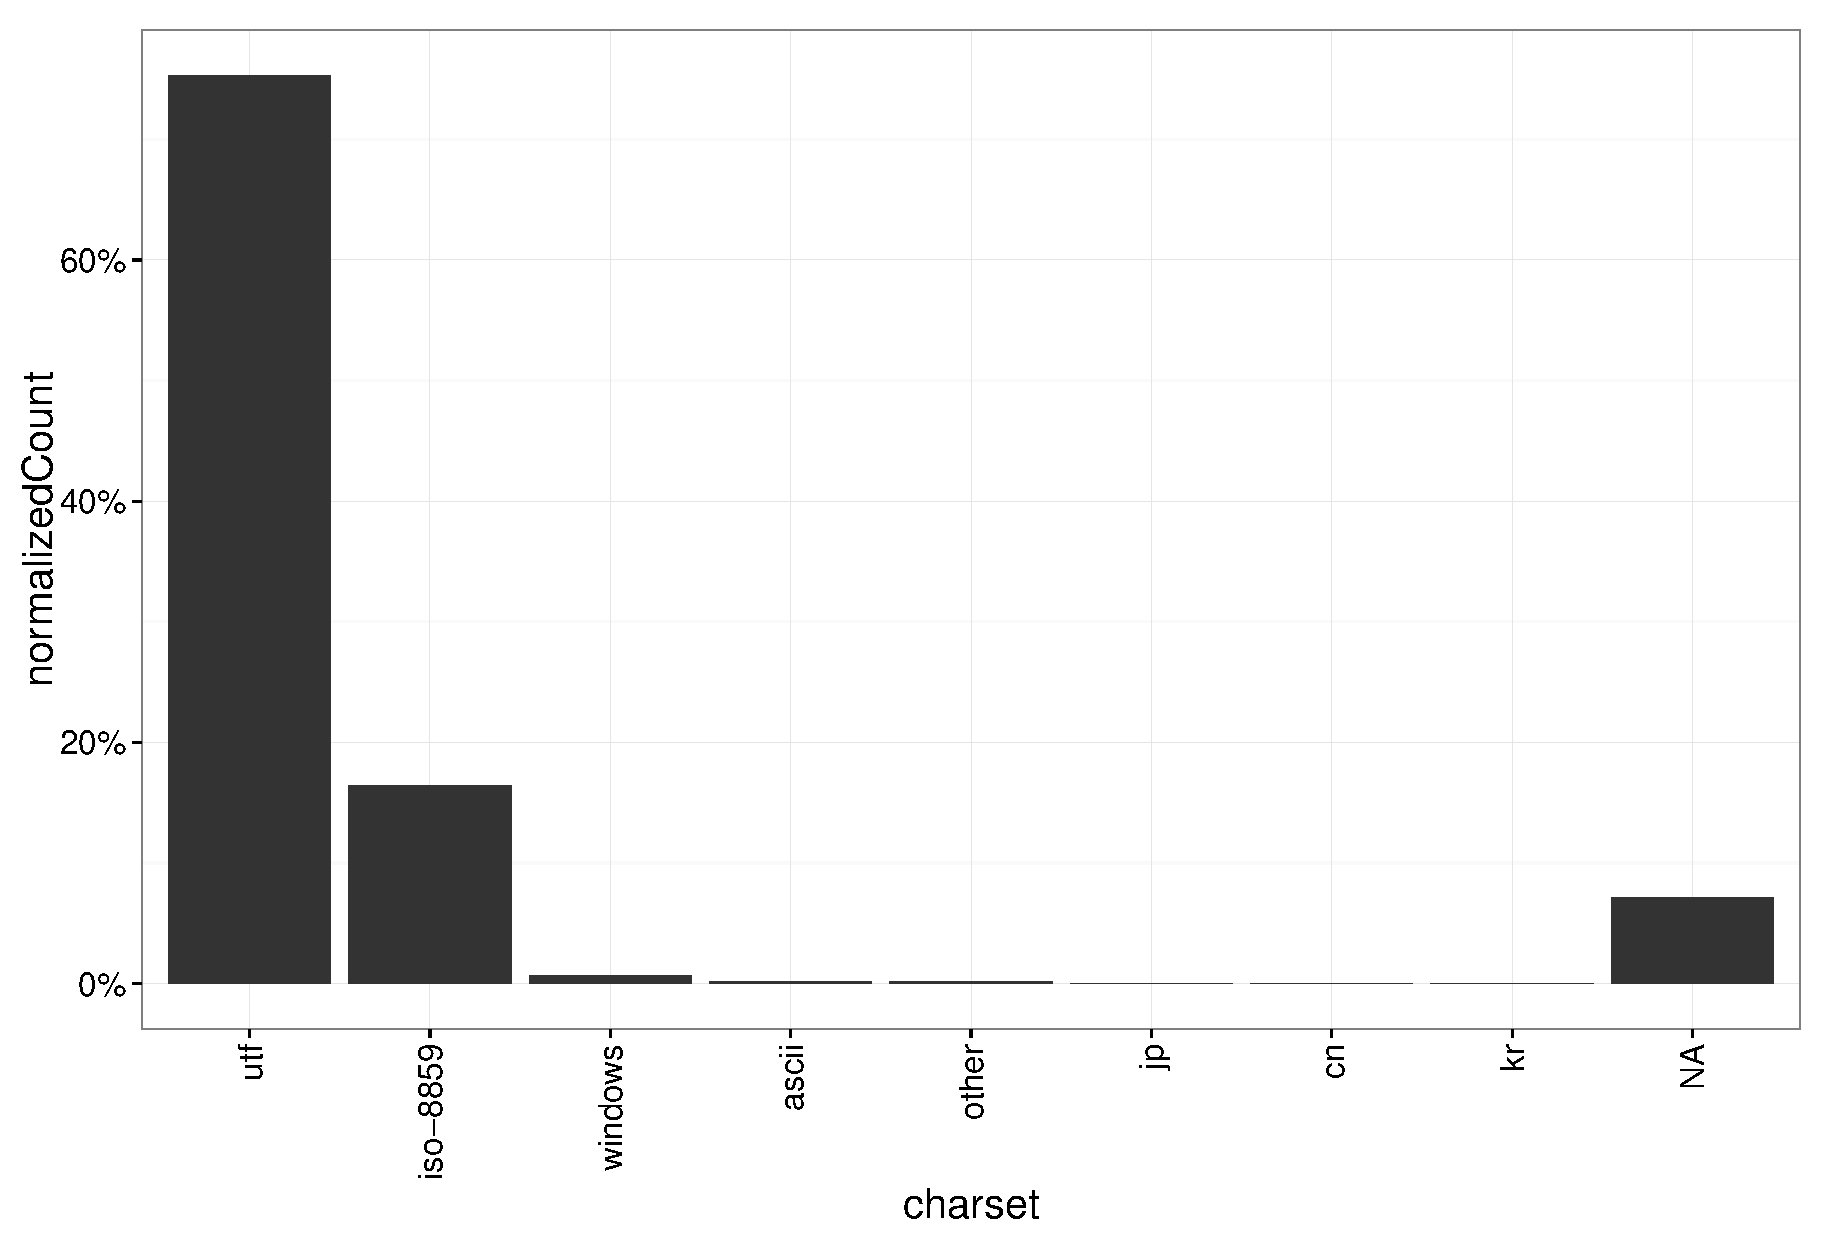
\includegraphics[width=.78\textwidth]{plots/plot_charset}
\end{center}

\noindent
Während ca. 16\% aller Seiten noch die regionsspezifischen Zeichenkodierungen des ISO-8859-Standards benutzen, setzt die große Mehrheit inzwischen auf Unicode.

Außerdem zeigt sich hier abermals, dass asiatische Seiten stark unterrepräsentiert sind, da die dort immer noch verwendeten Zeichenkodierungen wie die des JIS-Standards oder die Big5-Zeichenkodierung (im Graph nach Ländern gruppiert) quasi nicht auftreten.

\section{Webserver}

\begin{center}
    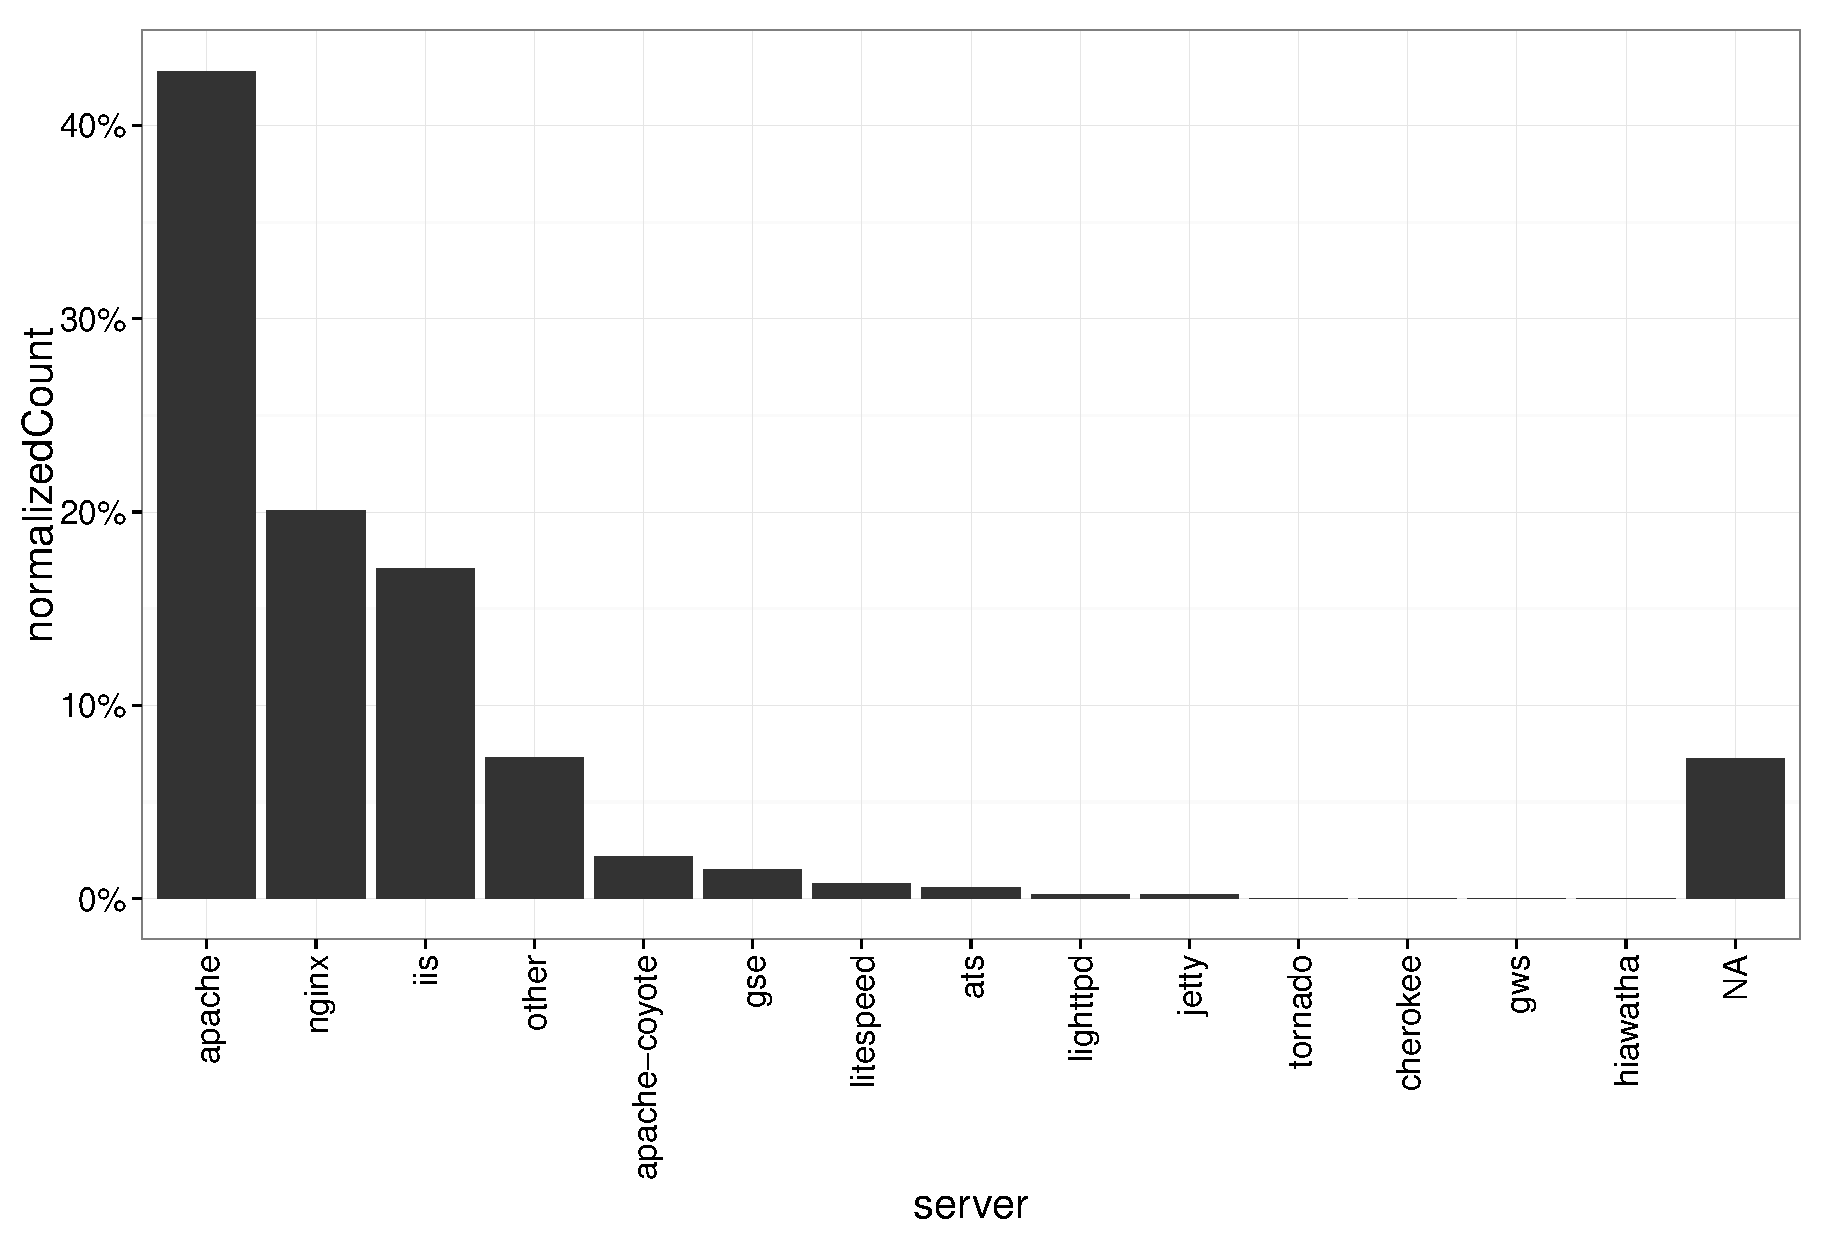
\includegraphics[width=.78\textwidth]{plots/plot_server}
\end{center}

\noindent
Bei den verwendeten Webservern herrscht eine große Vielfalt (vgl. den großen \texttt{other}-Anteil), die von den beiden großen freien Webservern Apache und nginx angeführt wird.

\section{Verschlüsselung, Cookies und Kompression}

\begin{center}
    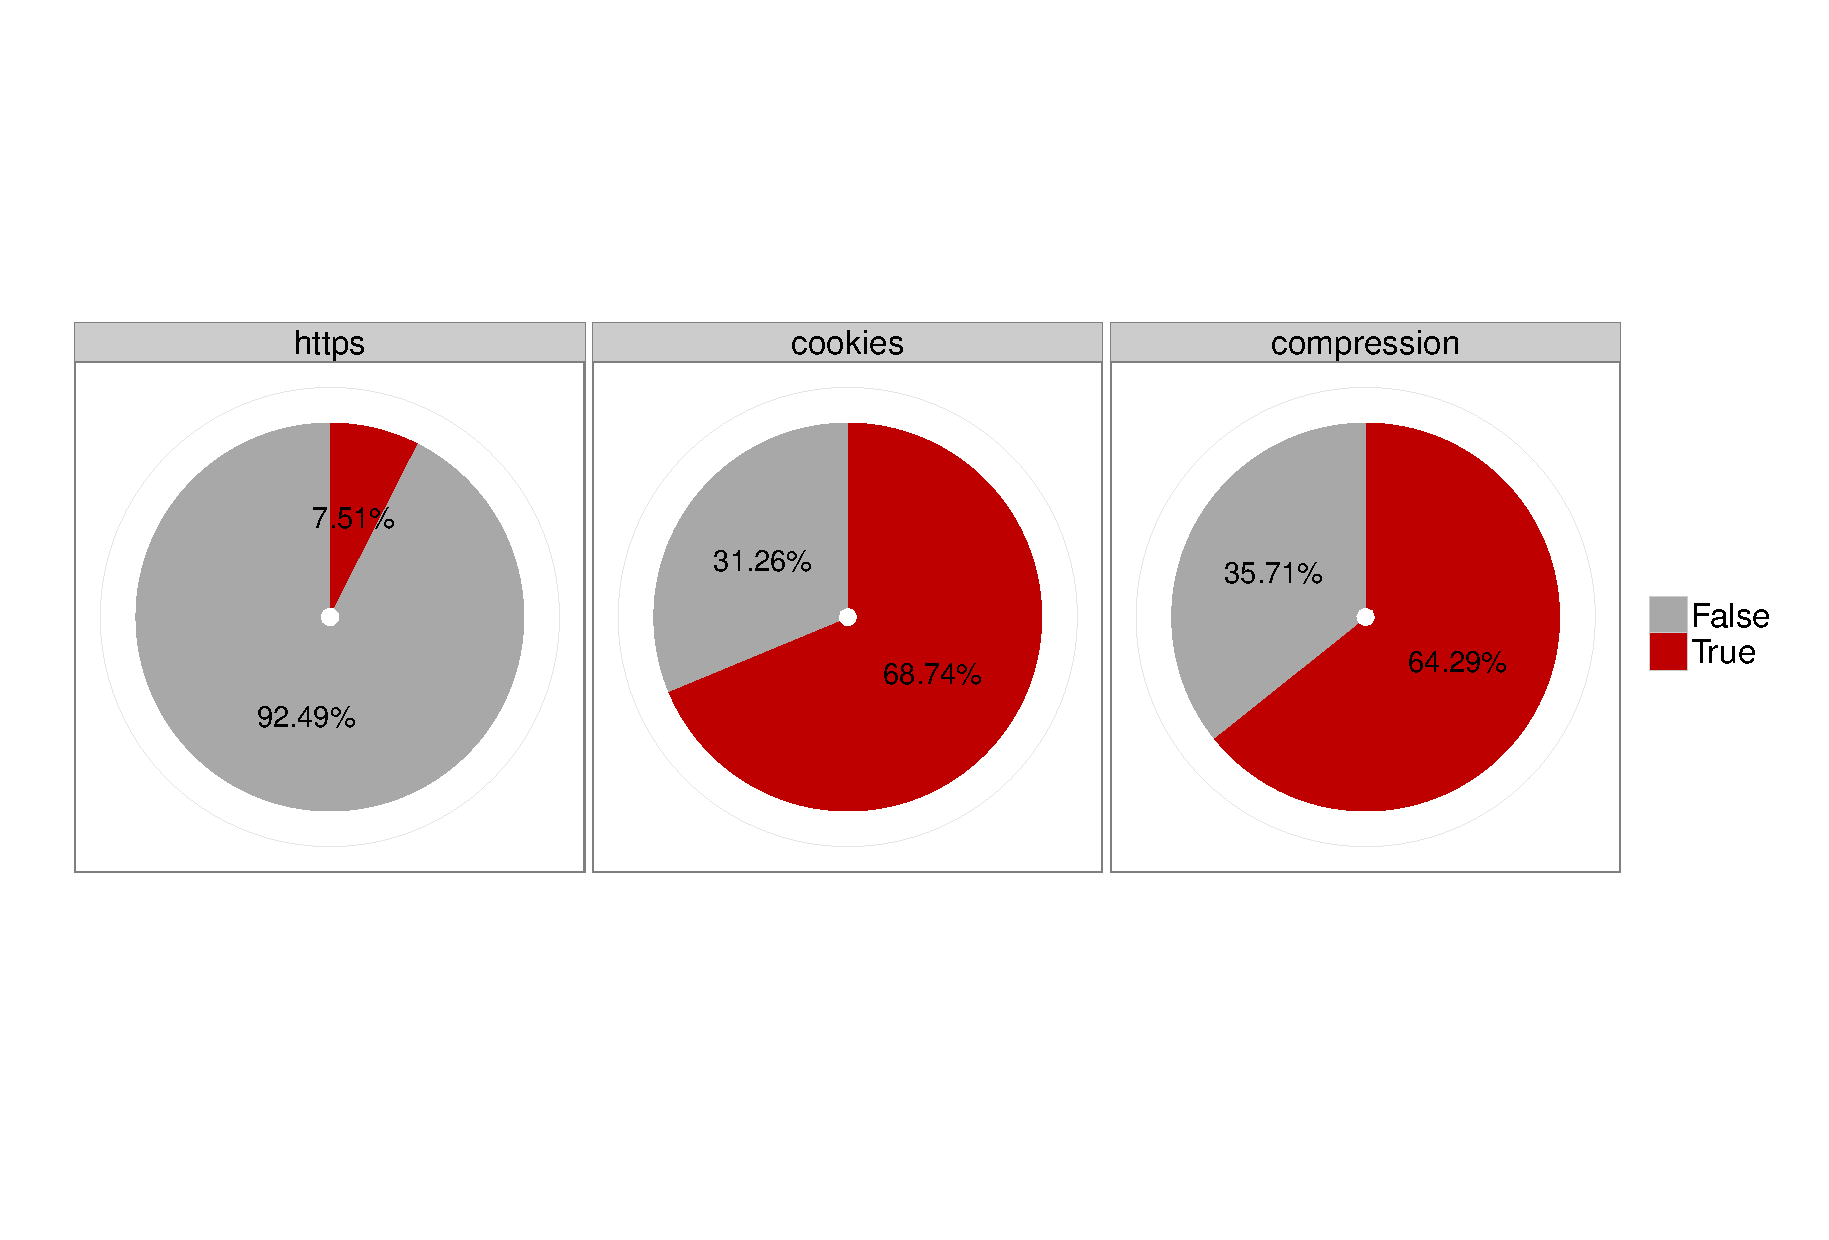
\includegraphics[trim=0 2cm 0 .5cm, clip=true, width=.9\textwidth]{plots/plot_boolean_pie}
\end{center}

\noindent
Mehr als 7\% der von Common Crawl gecrawlten Seiten verwenden HTTPS zur verschlüsselten Übertragung der Inhalte. Dies zeigt eindrucksvoll den seit ca. 4 Jahren anhaltenden Trend zur Verschlüsselung: 2011 lag der Anteil der verschlüsselten Seiten noch weit unter 1\%\footnote{%
\url{http://www.sistrix.de/news/anteil-von-ssl-treffern-google-serps/}}.

Im Gegensatz dazu versuchen mehr als zwei Drittel aller Seiten beim Besucher mindestens einen Cookie zu setzen. Es wurde hier jedoch nicht zwischen Session-Cookies und persistenten Cookies unterschieden.

Geringfügig weniger Seiten werden komprimiert (dh. mit \texttt{gzip} oder \texttt{deflate}) zum Browser übertragen.

\section{Links}

\makebox[\textwidth][c] {
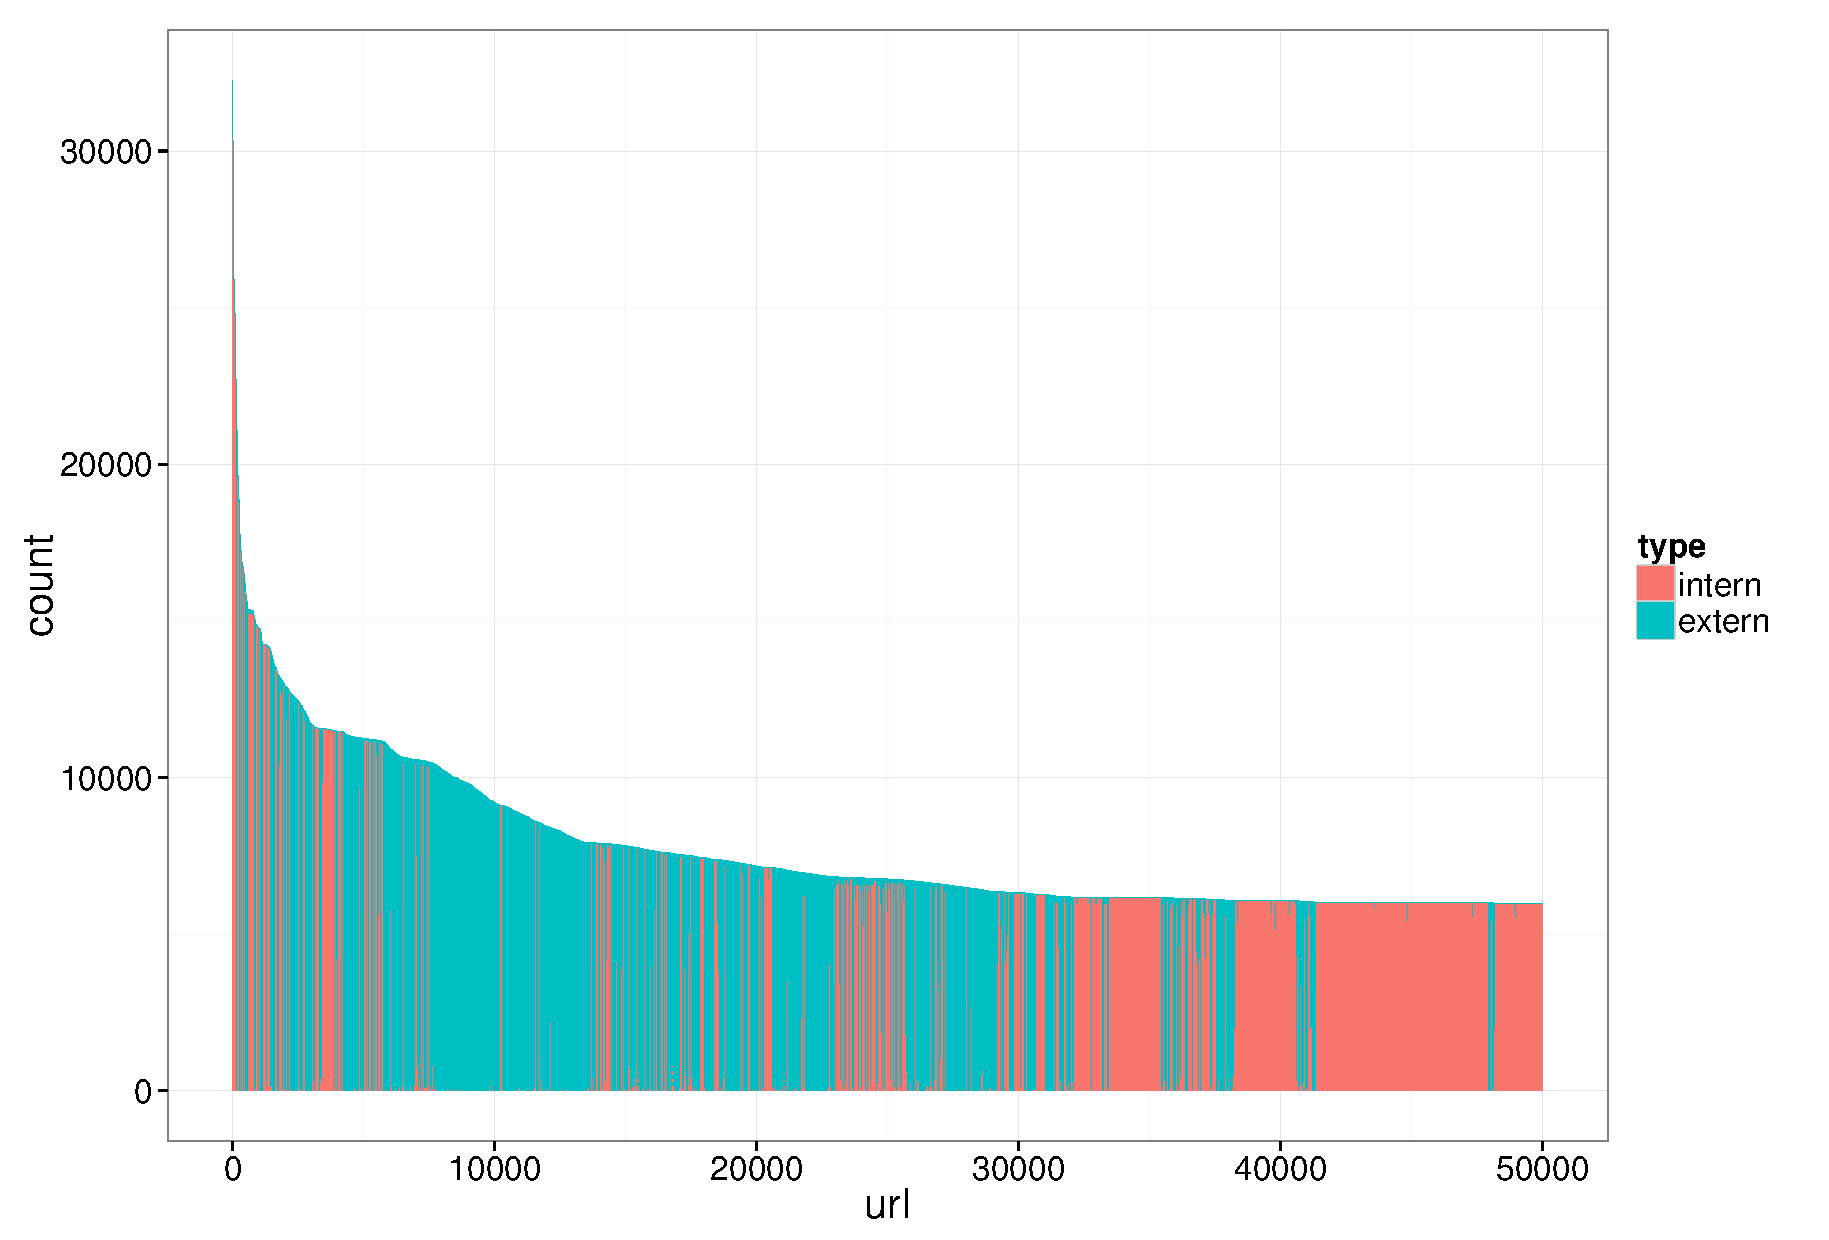
\includegraphics[trim=0 0 3.5cm 0, clip=true, width=0.39\textwidth, keepaspectratio=true]{plots/plot_links.pdf}%
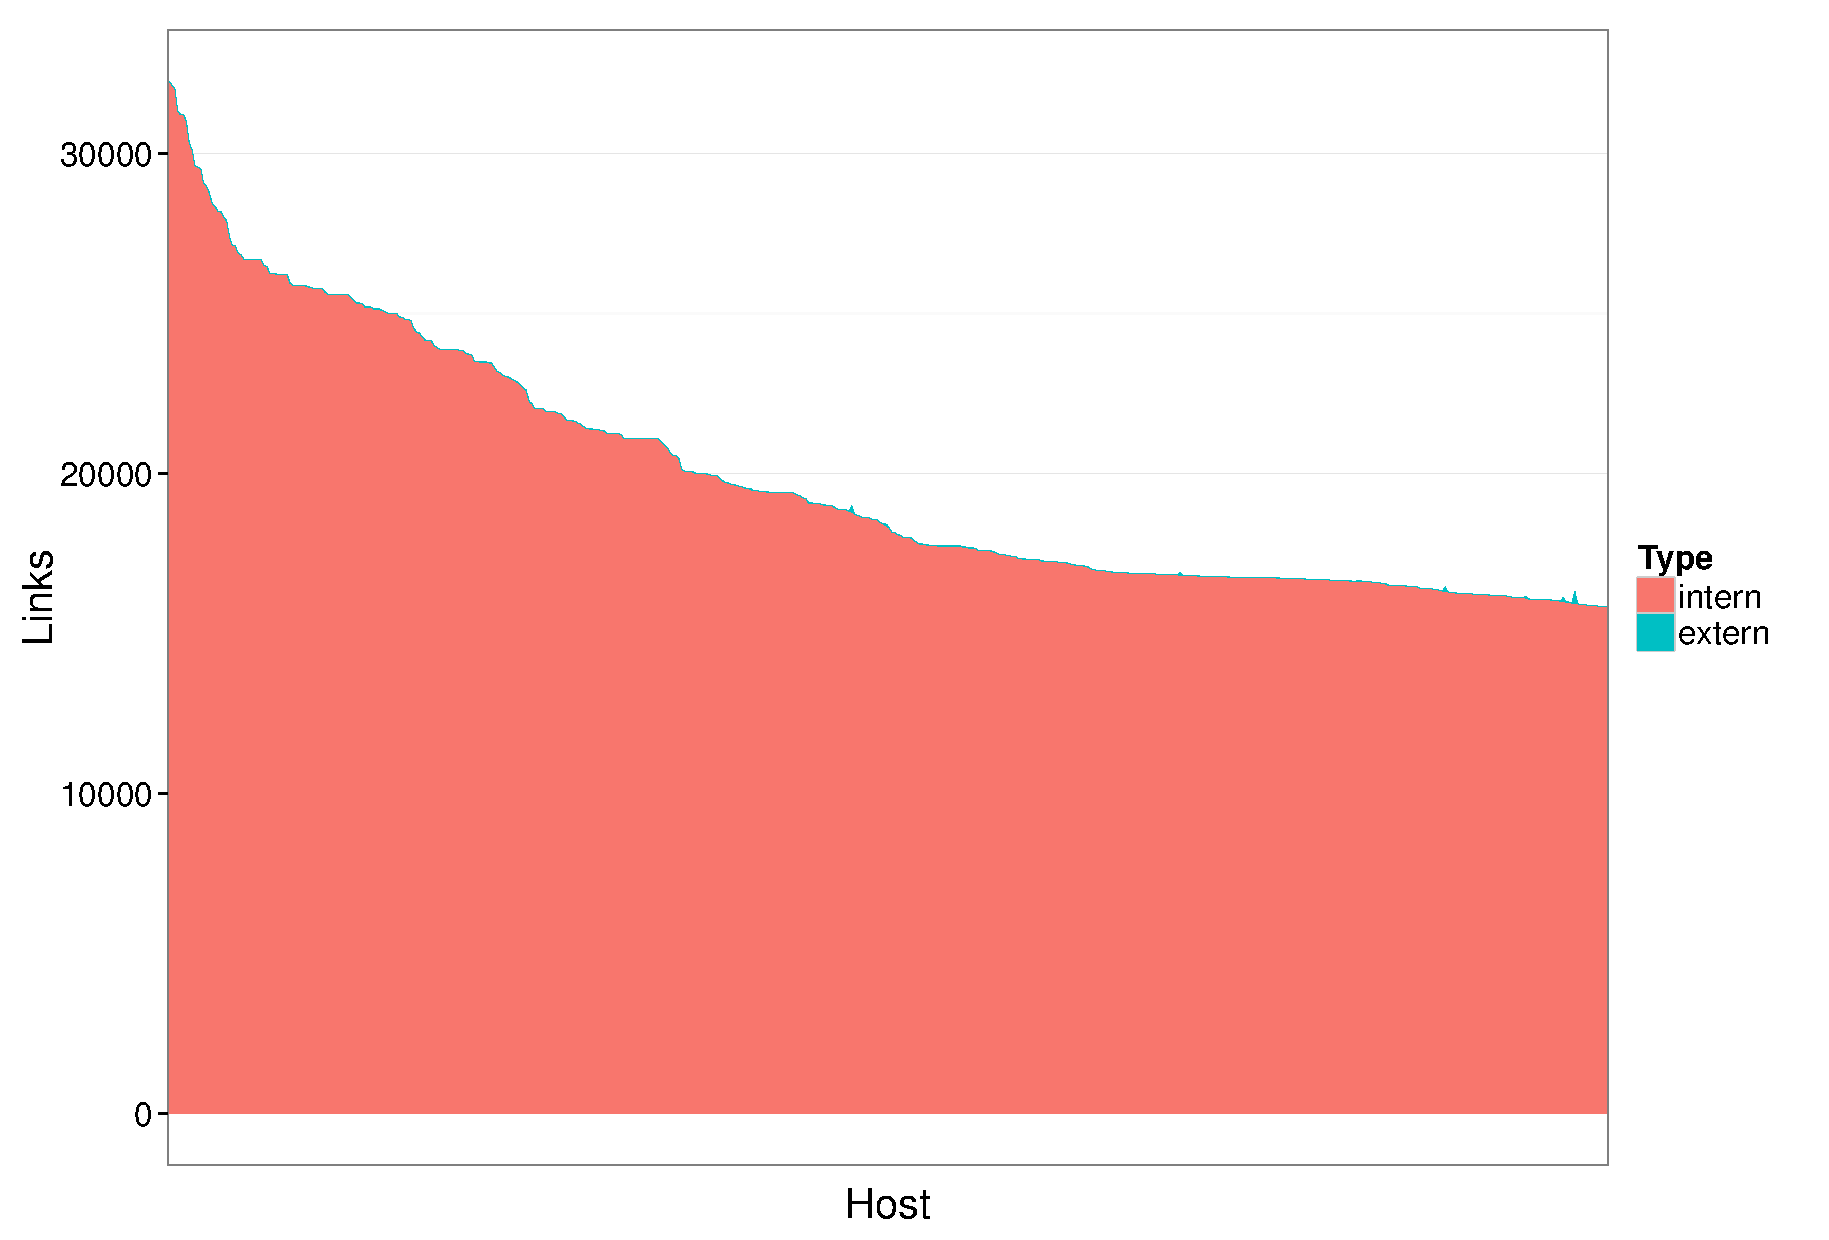
\includegraphics[trim=0 0 3.5cm 0, clip=true, width=0.39\textwidth, keepaspectratio=true]{plots/plot_links_internal.pdf}%
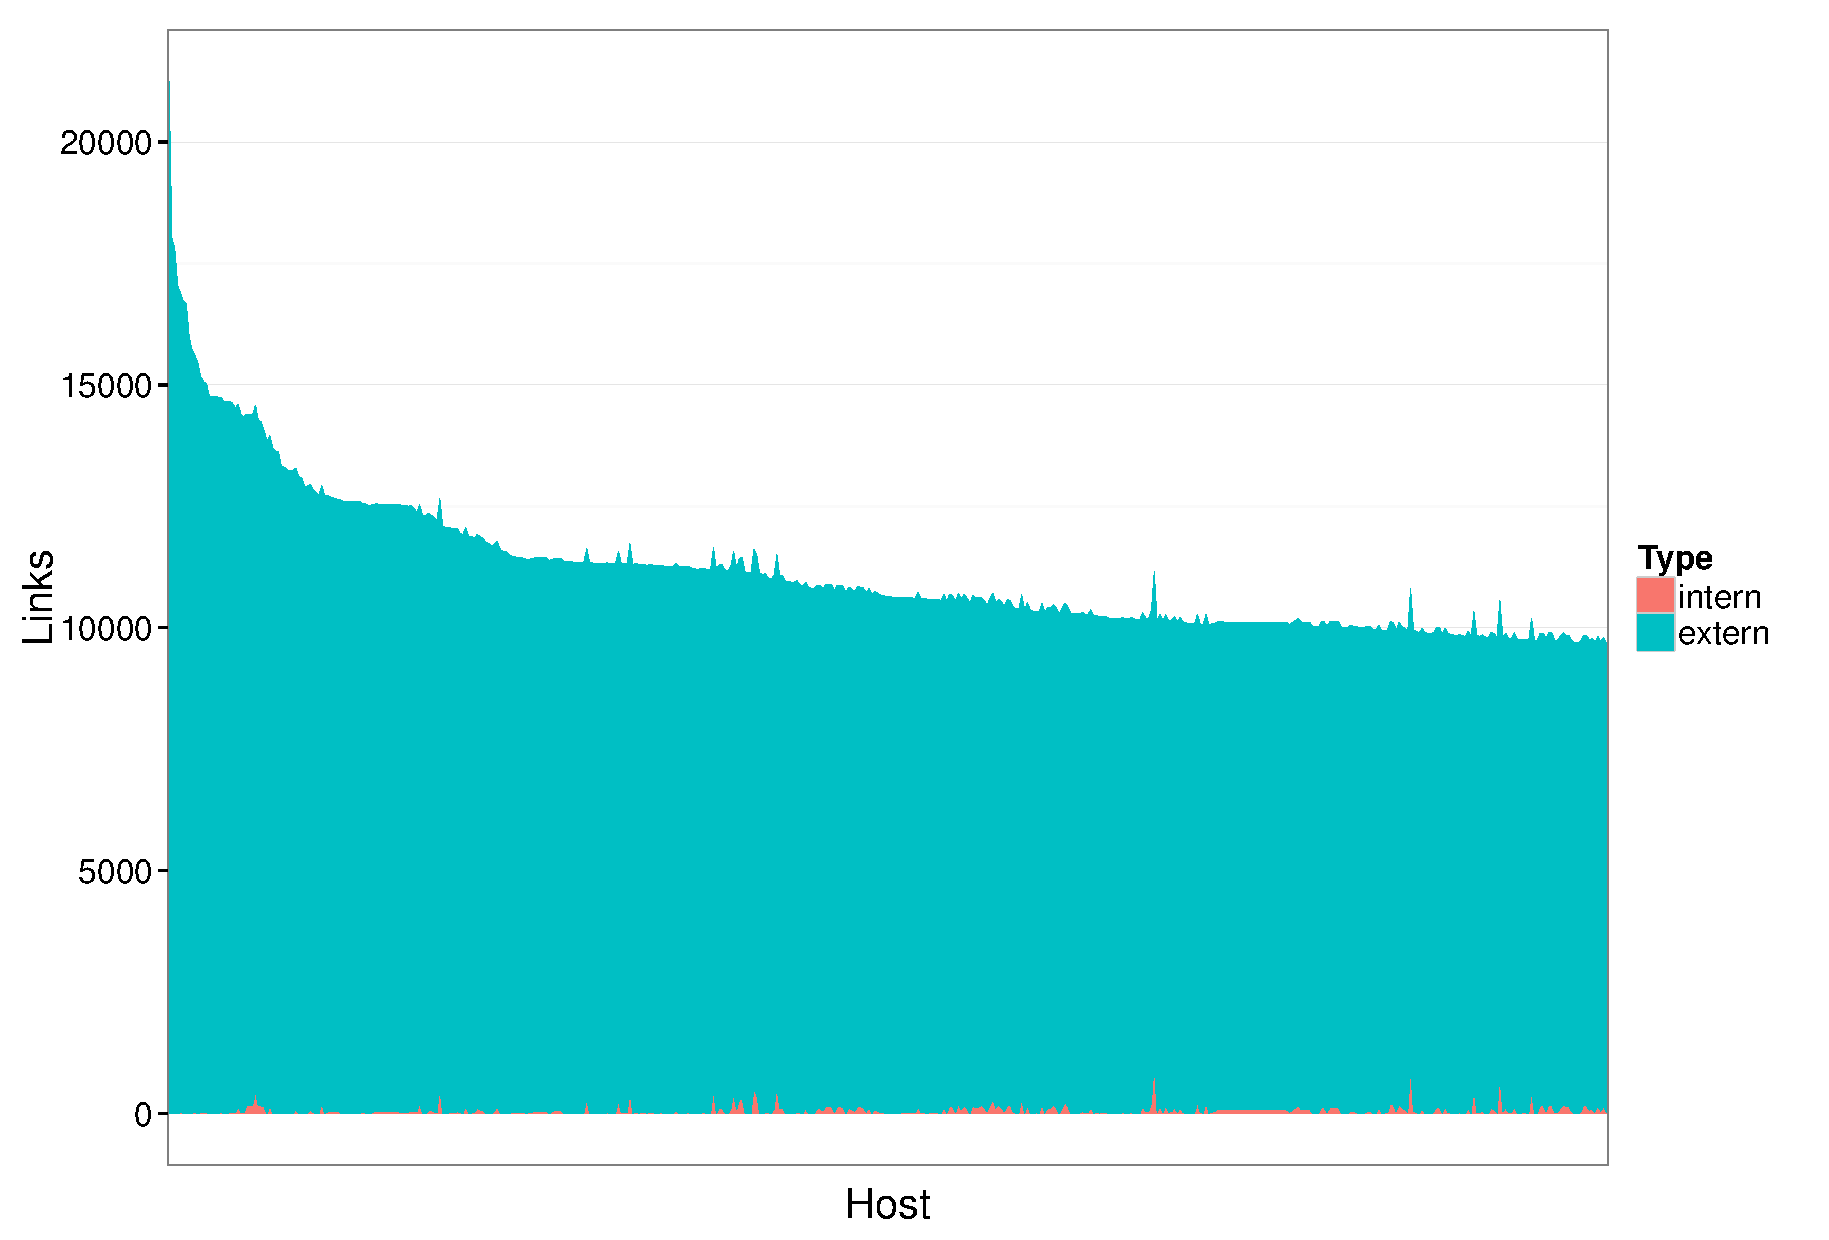
\includegraphics[trim=0 0 3.5cm 0, clip=true, width=0.39\textwidth, keepaspectratio=true]{plots/plot_links_external.pdf}
}
\centerline{Seiten mit den meisten (links), meisten internen (mitte, rot) und meisten externen (rechts, blau) Links}
\vspace{-.2cm}

Um die Reichweite des Crawls genauer zu beleuchten, betrachten wir die Verteilung und Art der Links, die auf den Seiten gefunden werden. Dabei unterscheiden wir zwischen internen Links, d.h. solche mit einem relativen Pfad bzw. mit dem gleichen Hostnamen als Ziel, und externen Links. In Bezug auf die Reichweite sind besonders externe Links interessant, da nur durch diese neue Seiten von anderen Hosts in den Crawl mit einbezogen werden.

Von allen Seiten enthalten etwa 84\% Links und 67\% externe Links. Ungefähr 18\% aller Links sind extern, der Rest verlinkt intern. Seiten mit sehr vielen externen/internen Links enthalten jedoch nahezu ausschließlich Links des selben Typs, die Verteilung ist eher asymmetrisch.

\section{Sprache}

\begin{center}
    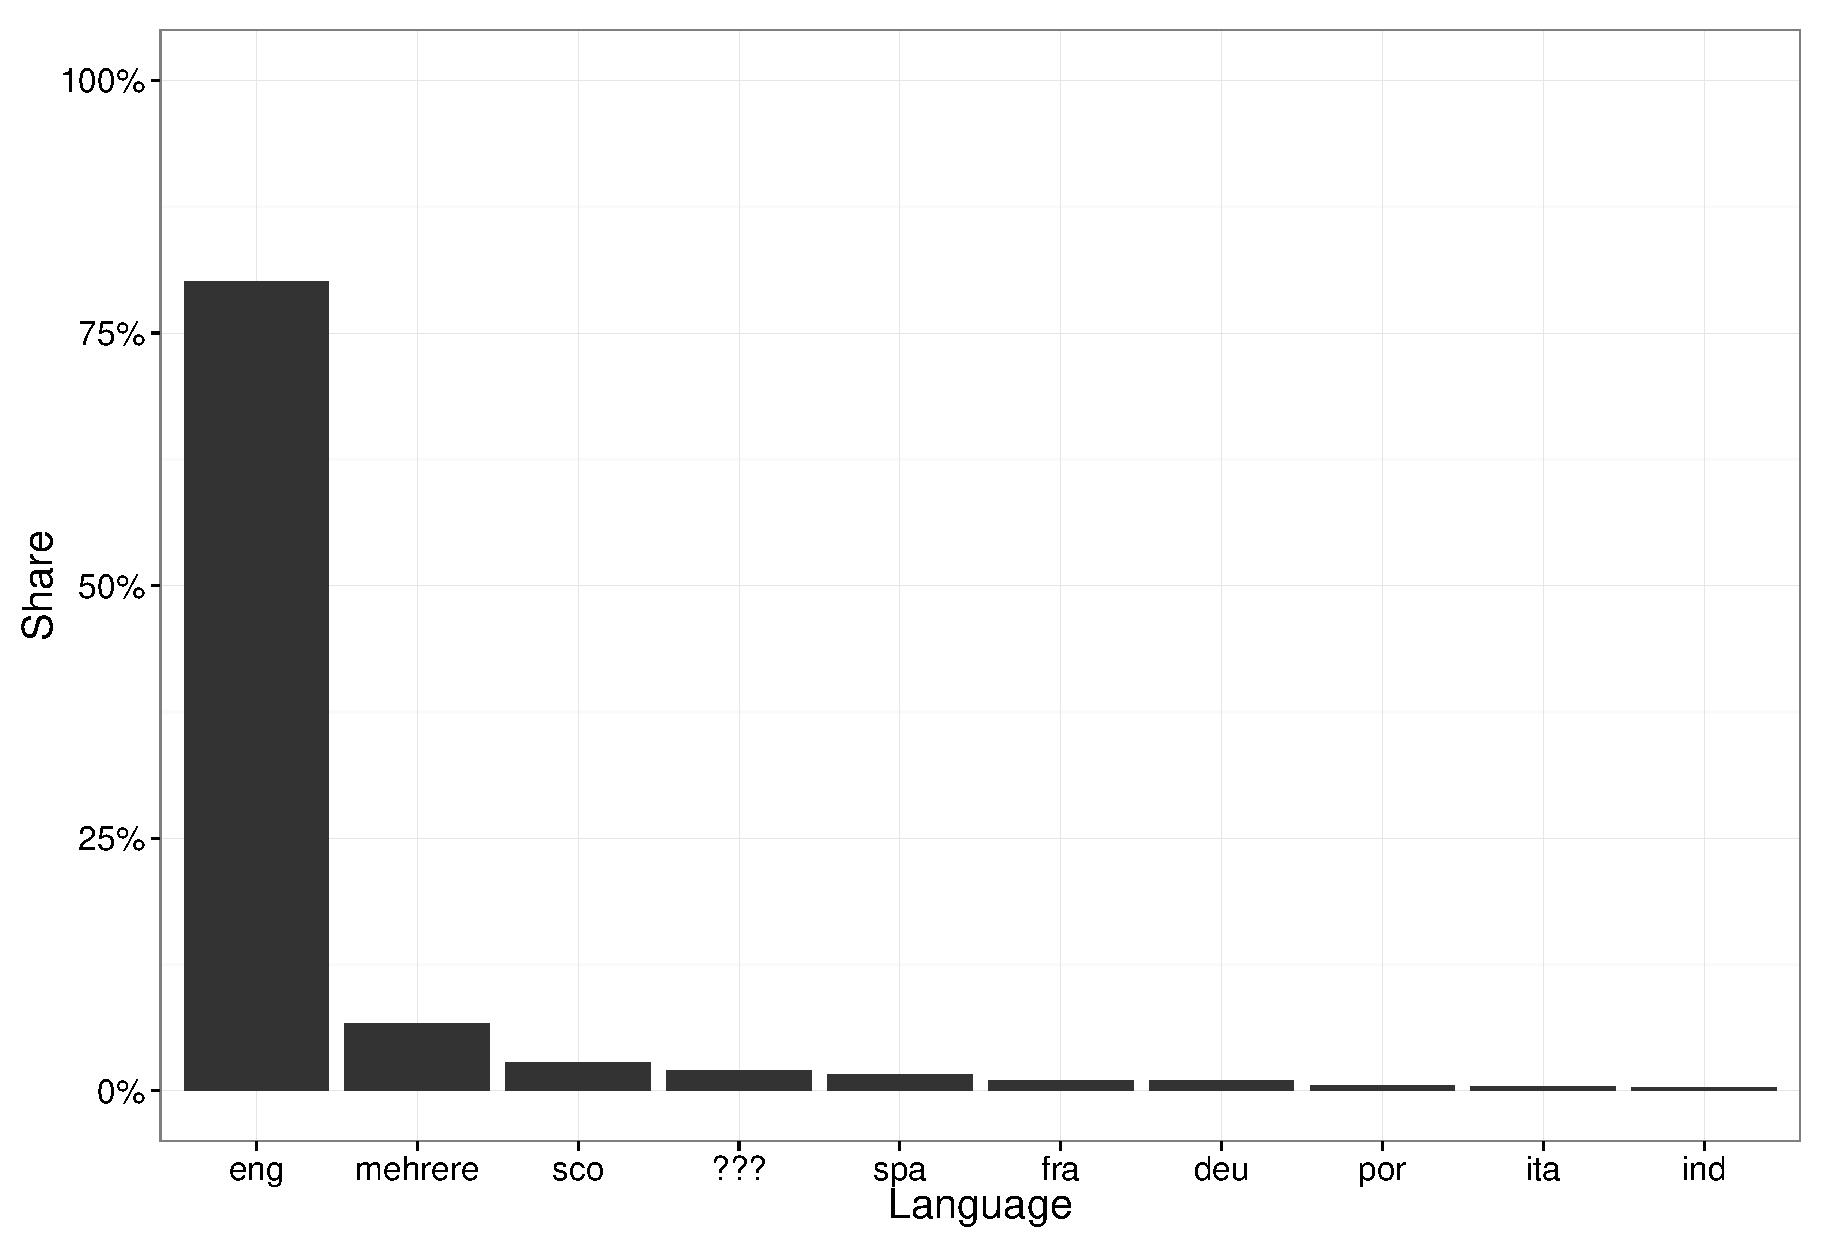
\includegraphics[width=.9\textwidth]{plots/plot_lang_top10}
\end{center}

Die Analyse der TLDs am Anfang des Kapitels kann nur einen groben Überblick über die Sprachverteilung geben. Aus diesem Grund wurde -- nach dem Vortrag -- zusätzlich zu den Metadaten auch ein Teil des eigentlichen Crawls analysiert. Dabei wurde eine zufällige Stichprobe mit 242 von insgesamt ca. 33000 WARC-Dateien (gepackt je ca. 1 GB) heruntergeladen und der Text extrahiert. Für die resultierenden knapp 11 Millionen Dokumente wurde anschließend mit dem LangSepa-Werkzeug der Fakultät jeweils die Sprache bestimmt.

Wie erwartet ist der Crawl sehr stark von Englisch dominiert. Die einzigen nicht-europäischen Sprachen innerhalb der ersten 20 (über 95 \% aller Dokumente) sind Indonesisch (3 \textperthousand), Vietnamesisch (1,7 \textperthousand) und Arabisch (1,6 \textperthousand). Koreanisch folgt auf Platz 24 mit 0,8 \textperthousand\ und Chinesisch auf Platz 31 mit 0,5 \textperthousand. Insgesamt wurden 367 verschiedene Sprachen erkannt.

\begin{wrapfigure}{r}{.57\textwidth}
    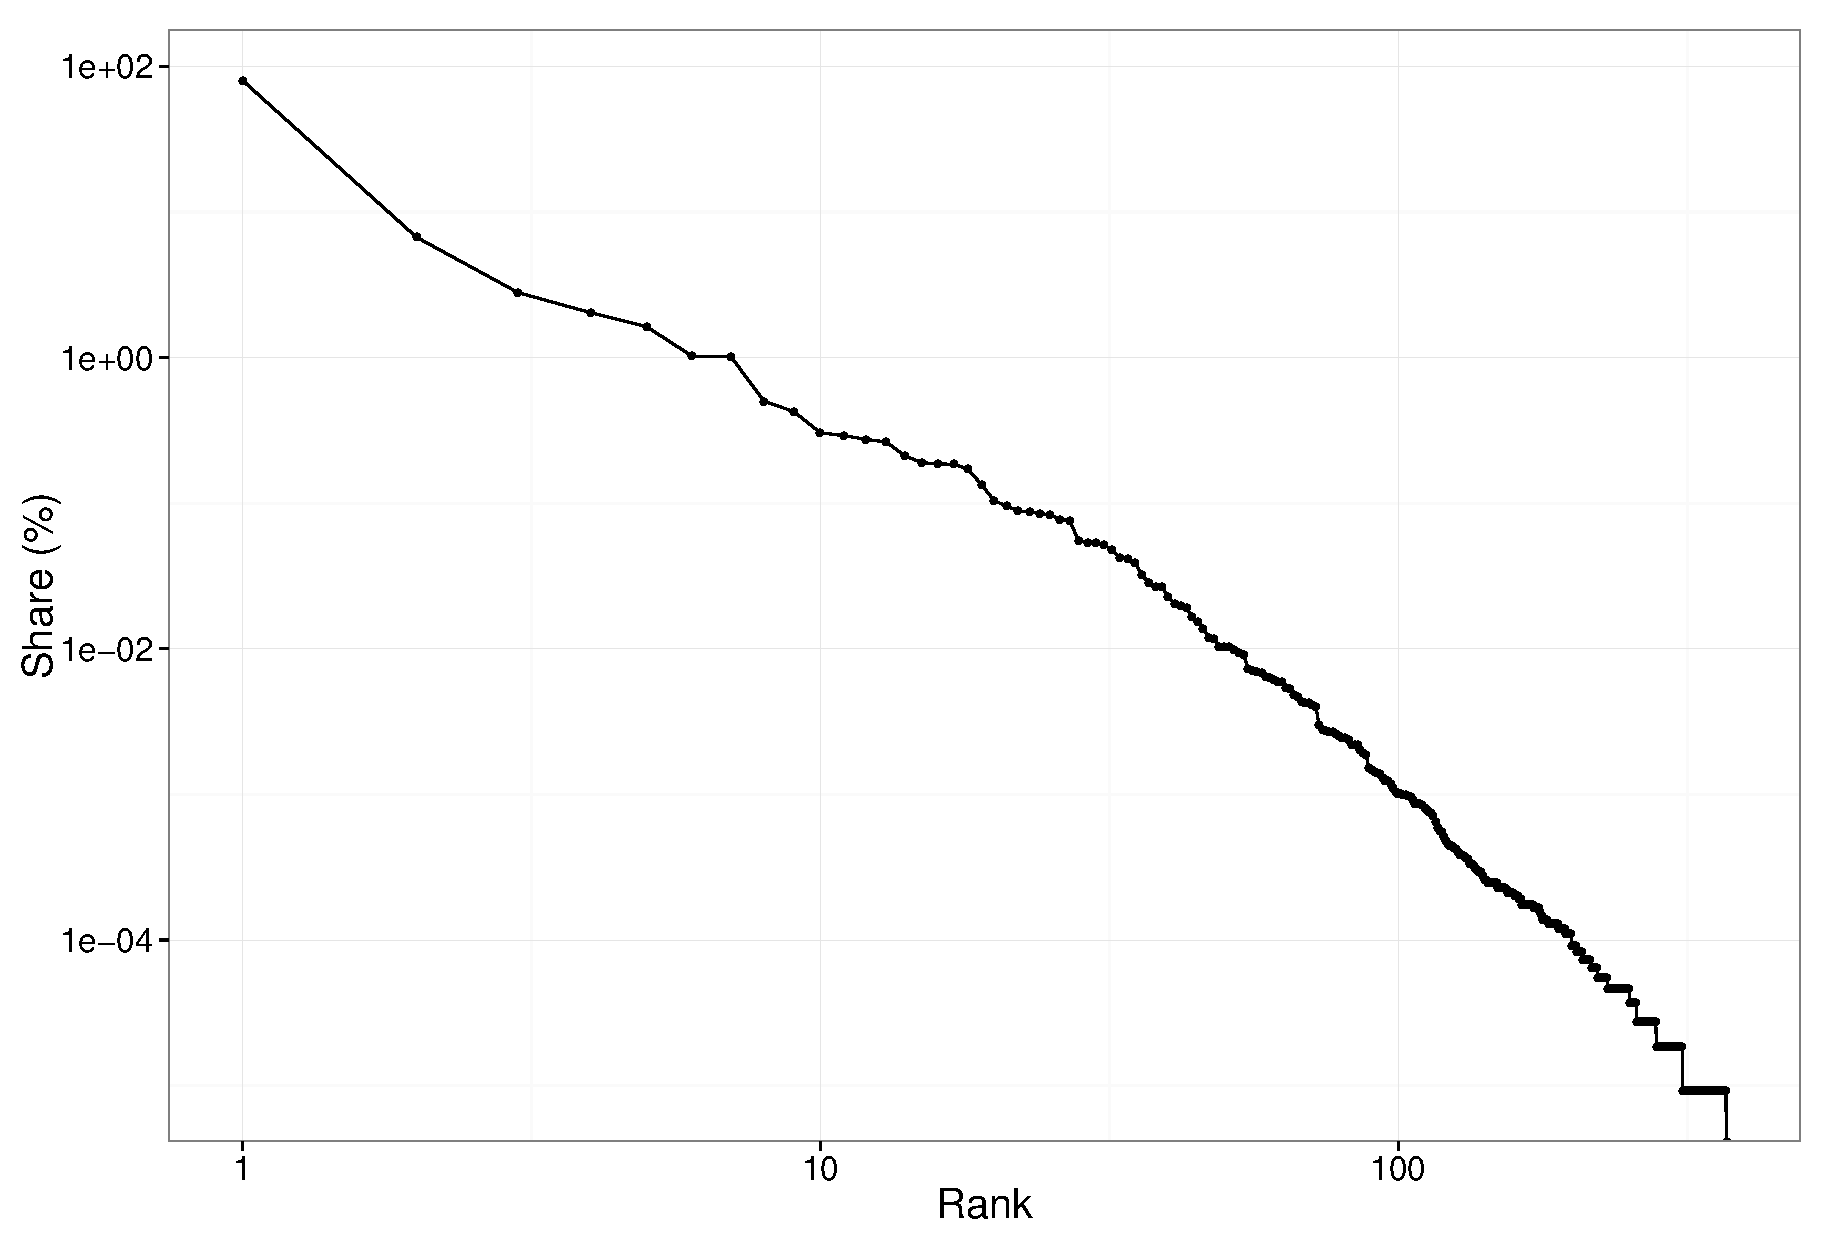
\includegraphics[width=.6\textwidth]{plots/plot_lang_log10.pdf}
\end{wrapfigure}

LangSepa scheint manchmal Probleme bei der Unterscheidung ähnlicher Sprachen zu haben. So haben Scots (27,9 \textperthousand) und das nigerianische Pidgin (1,9 \textperthousand) einen unrealistisch hohen Anteil. Da beide jedoch dem Englischen sehr ähnlich sind, kann man hier von einer Fehlklassifizierung eigentlich englischer Dokumente ausgehen.

Die Verteilung der Sprachen entspricht -- deutlicher noch als die der TLDs -- einer Zipf-Verteilung.


\chapter{Textextraktion}

In diesem Abschnitt vergleichen wir die Qualität der Textextraktion von Common Crawl mit dem an der Abteilung für Automatische Sprachverarbeitung der Universität Leipzig entwickelten Tool jWarcEx und Readability.js, das von Mozilla für die Leseansicht im Firefox-Browser verwendet wird.

Da wir uns bei der Analyse wie oben beschrieben auf die Metadaten beschränken mussten, erfolgte die Analyse stichprobenartig anhand einiger Beispiele, wovon im Folgenden zwei näher erläutert werden.

\section{Beispiel: theguardian.com}

Das erste Beispiel ist der erste Artikel von Glenn Greenwald, Ewen MacAskill und Laura Poitras über Edward Snowden auf \texttt{theguardian.com}\footnote{\url{http://www.theguardian.com/world/2013/jun/09/edward-snowden-nsa-whistleblower-surveillance}}:

\begin{center}
    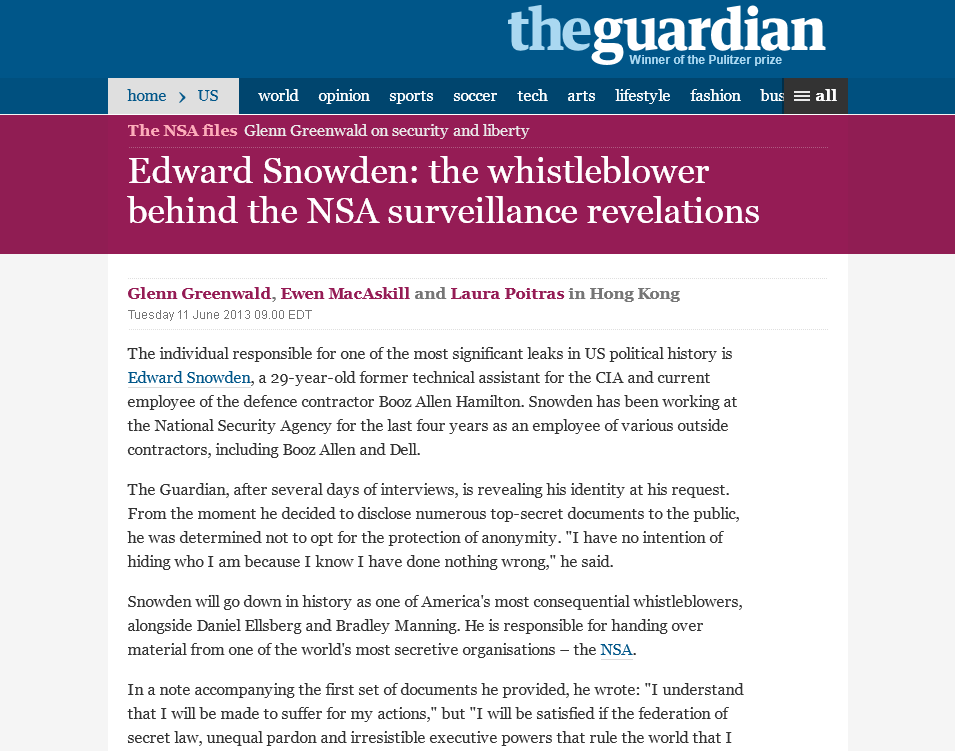
\includegraphics[trim=0 130px 0 0, clip=true, width=.8\textwidth]{images/guardian-website}
\end{center}

\noindent
Common Crawl und jWarcEx extrahieren in diesem Fall den exakt gleichen Text, der im Wesentlichen der DOM-Eigenschaft \texttt{textContent} entspricht und z.\,B. auch Elemente der Seitennavigation und Alternativtexte von Medien (vlg. Hinweis zum Video) enthält.

Readability.js extrahiert dagegen exakt den Text des Artikel. Die Überschrift und die Autoren werden aus den entsprechenden HTML-Meta-Tags entnommen, wobei hier fälschlicherweise nur das letzte author-Tag beachtet wird.

\begin{minipage}[t]{.5\textwidth}
    \centering{\textbf{Common Crawl / jWarcEx}}
    \vspace{.5cm}
    \scriptsize
    \begin{lstlisting}[breaklines=true]
    Skip to main content

    browse all sections close

    Glenn Greenwald on security and liberty

    Edward Snowden: the whistleblower behind the NSA surveillance revelations

    The 29-year-old source behind the biggest intelligence leak in the NSA's history explains his motives, his uncertain future and why he never intended on hiding in the shadows

    Q\&A with NSA whistleblower Edward Snowden: ``I do not expect to see home again''

    Glenn Greenwald, Ewen MacAskill and Laura Poitras in Hong Kong

    Tuesday 11 June 2013 09.00 EDT Last modified on Saturday 4 October 2014 10.54 EDT

    Sorry, your browser is unable to play this video.

    The individual responsible for one of the most significant leaks in US political history is Edward Snowden, a 29-year-old former technical assistant for the CIA and current employee of the defence contractor Booz Allen Hamilton. Snowden has been working at the National Security Agency for the last four years as an employee of various outside contractors, including Booz Allen and Dell.

    The Guardian, after several days of interviews, is revealing his identity at his request. From the moment he decided to disclose numerous top-secret documents to the public, he was determined not to opt for the protection of anonymity. "I have no intention of hiding who I am because I know I have done nothing wrong," he said.

    (...)
    \end{lstlisting}
\end{minipage}%
\begin{minipage}[t]{.5\textwidth}
    \centering{\textbf{Readability.js}}
    \vspace{.5cm}
    \scriptsize
    \begin{lstlisting}[breaklines=true]






    Edward Snowden: the whistleblower behind the NSA surveillance revelations










    Laura Poitras









    The individual responsible for one of the most significant leaks in US political history is Edward Snowden, a 29-year-old former technical assistant for the CIA and current employee of the defence contractor Booz Allen Hamilton. Snowden has been working at the National Security Agency for the last four years as an employee of various outside contractors, including Booz Allen and Dell.

    The Guardian, after several days of interviews, is revealing his identity at his request. From the moment he decided to disclose numerous top-secret documents to the public, he was determined not to opt for the protection of anonymity. "I have no intention of hiding who I am because I know I have done nothing wrong," he said.

    (...)
    \end{lstlisting}
\end{minipage}

\section{Beispiel: abc7.com}

Unterschiede zwischen der Textextraktion von Common Crawl und jWarcEx zeigen sich z.\,B. an einem Artikel über das Karriereende von Lance Armstrong auf \texttt{abc7.com}\footnote{\url{http://abc7.com/archive/7962461}}.

So erkennt jWarcEx die zu einem Menüpunkt gehörenden Unterpunkte und fasst diese zusammen, während Common Crawl damit teilweise Probleme hat. Außerdem fügt Common Crawl manchmal den Seitentitel an den Anfang des Extraktes hinzu.

\vspace{.5cm}
\begin{minipage}[t]{.5\textwidth}
    \centering{\textbf{Common Crawl}}
    \vspace{.5cm}
    \scriptsize
    \begin{lstlisting}[breaklines=true]
    Lance Armstrong, Tour de France champ, retires | abc7.com

    GO

    Personalize your weather by entering a location.

    Sorry, but the location you entered was not found. Please try again.

    Sections

    Traffic

    Video

    Los AngelesOrange CountyInland EmpireVentura CountyCalifornia

    Home

    Accuweather

    Traffic

    Video

    Photos

    Mobile Apps

    Local News Los AngelesOrange CountyInland EmpireVentura CountyCalifornia

    Map My News

    Shows Live Well Network

    Follow Us

    BREAKING NEWS

    (...)
    \end{lstlisting}
\end{minipage}%
\begin{minipage}[t]{.5\textwidth}
    \centering{\textbf{jWarcEx}}
    \vspace{.5cm}
    \scriptsize
    \begin{lstlisting}[breaklines=true]





    Personalize your weather by entering a location.

    Sorry, but the location you entered was not found. Please try again.

    Sections Traffic Video Los AngelesOrange CountyInland EmpireVentura CountyCalifornia






    Home Accuweather Traffic Video Photos Mobile Apps










    Los AngelesOrange CountyInland EmpireVentura CountyCalifornia







    BREAKING NEWS ABC shows live and on-demand -- Download the WATCH ABC app!

    (...)
    \end{lstlisting}
\end{minipage}

\end{document}
